\documentclass{beamer}
% This is the file main.tex
%\usetheme{default}
\usetheme{CambridgeUS}
%\usecolortheme{seahorse}
\usecolortheme{rose}
\usefonttheme[onlylarge]{structuresmallcapsserif}
\usefonttheme[onlysmall]{structurebold}
%\setbeamerfont{title}{shape=\itshape,family=\rmfamily}
%\setbeamercolor{title}{fg=red!80!black}
%\setbeamercolor{title}{fg=red!80!black,bg=red!20!white}

% Utilizamos el paquete para usar español
%\usepackage[spanish]{babel}
% Utilizamos un paquete para gestionar los acentos
% y las e ¿es
%\usepackage[utf8]{inputenc}
% amsmath y amssymb de la American Mathematical 
% Society (f\'ormulas matem\'aticas)
\usepackage{amsmath}
\usefonttheme[onlymath]{serif}
%Para que reconozca el entorno verbatim
\usepackage{fancyvrb}
%Definimos nuestra ruta para las imagenes
%Absoluto
%\graphicspath{ {/home/user/images/} }
%Relativo (recomendado) -> seg\'un
%https://es.sharelatex.com/learn/Inserting_Images#La_ruta_a_la_carpeta_de_im.C3.A1genes
\graphicspath{ {media/} }


\title[]{SiPM: a novel photon detector becoming a classic}
\subtitle{School and Workshop on Dark Matter and Neutrino Detection \\ San
Pablo, Brazil \\ ICTP-SAIFR/IFT-UNESP}
\author[\texttt{@horacio\_arnaldi}]{Horacio Arnaldi \\ \texttt{{\href{mailto:arnaldi@cab.cnea.gov.ar}{arnaldi@cab.cnea.gov.ar}}}}
\institute[LabDPR - CAB - IB]{Laboratorio Detecci\'on de Part\'iculas y
Radiaci\'on \\ Centro At\'omico Bariloche - Instituto Balseiro}
%\date{\today}
\date{}

\begin{document}

\begin{frame}
\hspace*{0.6cm}
\includegraphics[height=0.18\textheight]{logos/cnea_logo} \hspace*{1cm}
\includegraphics[height=0.18\textheight]{logos/balseiro_logo} \hspace*{1cm}
\includegraphics[height=0.18\textheight]{logos/LabDPR_logo} \hspace*{1cm}
\includegraphics[height=0.18\textheight,width=0.15\textwidth]{logos/lagologo}

\titlepage

\end{frame}

\begin{frame}
\frametitle{Outline}
\setcounter{tocdepth}{1} %para incluir solo las secciones en el TOC
\tableofcontents
%  \tableofcontents[pausesections]
\end{frame}

%------------------------------------------------------------------------------
\section{Introducci\'on}
%------------------------------------------------------------------------------

\begin{frame}
\begin{center}
\Huge{\color{blue}{Introducci\'on}}
\end{center}
\end{frame}

\begin{frame}
\frametitle{Introducci\'on}
\only<1>{\fbox{\includegraphics[width=\textwidth]{d1/block_diag_det_syst}}}
\only<2>{\fbox{\includegraphics[width=\textwidth]{d1/block_diag_det_syst1}}}
\end{frame}

%FIXME: ver si incluir el principio del Knoll donde habla de fuentes de radiaci\'on, como para entrar en contexto de qu\'e es lo que queremos medir
\begin{frame}
\begin{block}{Introducci\'on}
\begin{itemize}
\item Describiremos y definiremos algunas catacter\'isticas generales, comunes a los
detectores, las señales y el ruido asociado a ellos
\item Principio fundamental: \alert{La transferencia de parte o toda la energ\'ia
de radiaci\'on a la masa del detector donde es convertida a otra forma m\'as
accesible para la percepci\'on humana}
\item Las part\'iculas cargadas transfieren su energ\'ia a la materia a trav\'es de
colisiones directas con los electrones at\'omicos, induciendo
{\color{blue}excitaci\'on} o {\color{blue}ionizaci\'on} en los \'atomos
\item La radiaci\'on neutra, por otro lado, primero debe producir alg\'un tipo de
reacci\'on en el detector producciendo part\'iculas cargadas, las cuales a su vez
ionizan y excitan los \'atomos del detector
\end{itemize}
\end{block}
\end{frame} 

\begin{frame}
\begin{block}{Introducci\'on (cont.)}
\begin{itemize}
\item La forma en la que la energ\'ia convertida aparece {\color{blue}depende del detector y de
su diseño}
\item Los detectores modernos de hoy en d\'ia son esencialmente
el\'ectricos/electr\'onicos
\item En alg\'un punto la informaci\'on proveniente del detector es
tranformada a pulsos el\'ectricos, los cuales pueden tratarse con t\'ecnicas
electr\'onicas
\item Cuando hablamos de ``detectores'' estamos, entonces, teniendo en cuenta su
electr\'onica asociada tambi\'en
\end{itemize}
\end{block}
\end{frame} 

\begin{frame}
\frametitle{Elecci\'on del detector}
\begin{alertblock}{Factores de decisi\'on}
\begin{itemize}
\item La regi\'on de longitudes de onda de la radiaci\'on 
\item La intensidad de la radiaci\'on
\item La respuesta temporal requerida para resolver eventos de alta
velocidad
\item La superficie de detector requerida
\item El ambiente en el cual el detector ser\'a usado
\item El costo
\item La electr\'onica asociada al detector
\end{itemize}
\end{alertblock}
\end{frame} 

%esta parte sigue los lineamientos de Spieler Introducci\'on
%------------------------------------------------------------------------------
\subsection{¿Por qu\'e?}
%------------------------------------------------------------------------------

\begin{frame}
\frametitle{¿Por qu\'e?}
{
\setbeamercolor{block body}{bg=red!20, fg=blue}
\begin{block}{}
La radiaci\'on es el \'unico {\color{red}observable} en procesos que ocurren en una escala que es
demasiado breve o demasiado pequeña para ser observada directamente. Tambi\'en es
el \'unico acceso a procesos que est\'an muy lejos.
\end{block}
}
\begin{block}{}
Originalmente desarrollado para la f\'isica de part\'iculas at\'omica, nuclear y
elemental, los detectores de radiaci\'on ahora se aplican en muchas \'areas diversas
de la ciencia, la ingenier\'ia y la vida cotidiana.
\end{block}
{
\setbeamercolor{block body}{bg=green!20}
\begin{block}{}
El progreso en la ciencia no s\'olo es impulsado por la interacci\'on de la teor\'ia y
el experimento, sino tambi\'en por los avances en la {\color{blue}instrumentaci\'on}
\end{block}
}
\end{frame}

\begin{frame}
\frametitle{Tipos de radiaci\'on}
\begin{alertblock}{}
\begin{itemize}
\item[a] Part\'iculas cargadas 
\begin{itemize}
\item {\color{blue}electrones, protones, n\'ucleos at\'omicos, part\'iculas
elementales} 
\end{itemize}
\item[b] Part\'iculas neutras 
				\begin{itemize}
\item {\color{blue}neutrones, part\'iculas elementales, gravitones
elementales} 
				\end{itemize}
\item[c] Fotones 
				\begin{itemize}
\item {\color{blue}ondas milim\'etricas, rayos gamma, rayos X, luz
elementales} 
				\end{itemize}
				\end{itemize}
				\end{alertblock}
				\end{frame}

				\begin{frame}
\frametitle{La mayor\'ia de los detectores modernos convierten la
energ\'ia absorvida en una señal el\'ectrica}
\begin{alertblock}{La sensibilidad de la detecci\'on depende de:}
\begin{itemize}
\item fluctuaciones en el detector
\item fluctuaciones en la electr\'onica
\end{itemize}
\end{alertblock}
\begin{exampleblock}{Para maximizar la sensibilidad en la detecci\'on se
deben considerar:}
\begin{itemize}
\item la formaci\'on de la señal en el detector
\item el acoplamiento del detector a la electr\'onica
\item las fluctuaciones en la electr\'onica
\end{itemize}
\end{exampleblock}
\end{frame}

\begin{frame}
\frametitle{\small{El desarrollo de sistemas detectores es una mezcla interdisciplinaria de f\'isica y electr\'onica}}
{
\setbeamercolor{block body}{bg=blue!20}
\small{Por ejemplo, la comprensi\'on de un detector moderno de tracking
(seguimiento) en f\'isica de altas energ\'ias o de un sistema de im\'agenes m\'edicas
requiere conocimientos de:}
\begin{itemize}
\item f\'isica de estado s\'olido
\item f\'isica de dispositivos semiconductores
\item tecnolog\'ia de fabricaci\'on de semiconductores
\item t\'ecnicas para electr\'onica de bajo ruido
\item microelectr\'onica anal\'ogica y digital
\item transmisi\'on de datos a altas velocidades
\item sistemas de adquisici\'on de datos basados en computadoras
\end{itemize}
}
\begin{exampleblock}{}
\small{¡Es decir que es una gran forma de aprender sobre la interrelaci\'on de la
\alert{f\'isica} con la \alert{tecnolog\'ia}!}
\end{exampleblock}
\end{frame}

%------------------------------------------------------------------------------
\subsection{Ejemplos}
%------------------------------------------------------------------------------

%------------------------------------------------------------------------------
\subsection{El problema}
%------------------------------------------------------------------------------

\begin{frame}
\frametitle{El problema}
\begin{alertblock}{}
\begin{itemize}[<+->]
\item La radiaci\'on afecta a un sensor y genera una señal el\'ectrica

\item El nivel de señal es bajo y debe amplificarse para permitir la digitalizaci\'on y
el almacenamiento

\item Tanto el sensor como los amplificadores introducen fluctuaciones de señal/ruido
\begin{enumerate}
\item Fluctuaciones en la señal introducida por el sensor
\item Ruido de la electr\'onica superpuesta a la señal
\end{enumerate}

\item El l\'imite de detecci\'on y la precisi\'on de la medici\'on est\'an
determinados por la relaci\'on señal/ruido (SNR)
\end{itemize}
\end{alertblock}

\only<7>{\begin{alertblock}{¿C\'omo optimizar la relaci\'on señal/ruido?}
\begin{enumerate}
\item Aumentar la señal y reducir el ruido
\item Para un sensor y una señal dada: {\color{blue}reducir el ruido
electr\'onico}
\end{enumerate}
\end{alertblock}}
\end{frame}

\begin{frame}
\frametitle{Ejemplo}
\begin{block}{}
\includegraphics[height=0.35\textheight,width=\textwidth]{d1/espectro_pulso_unipolar} \\
\includegraphics[height=0.35\textheight,width=\textwidth]{d1/espectro_pulso_bipolar} 
\end{block}
\end{frame} 

\begin{frame}
\frametitle{\small{El espectro de ruido generalmente es distinto al de la
señal}}
\begin{columns}
\begin{column}{0.5\textwidth}
\begin{block}{\small{Espectro de ruido t\'ipico}}
\includegraphics[height=0.4\textheight,width=\textwidth]{d1/espectro_ruido_tipo}
\end{block}
\end{column}
\begin{column}{0.48\textwidth}
\begin{alertblock}{}
Adaptar la respuesta en frecuencia del sistema de medici\'on para optimizar la
relaci\'on señal/ruido
\end{alertblock}
\end{column}
\end{columns}
\begin{block}{}
La respuesta en frecuencia del sistema de medici\'on \alert{afecta a los dos}: señal y
ruido
\end{block}
\end{frame} 

\begin{frame}
\frametitle{Pasos para el an\'alisis de un sistema de procesamiento de pulsos}
\begin{exampleblock}{}
\begin{itemize}
\item Determinar la magnitud de la señal y su dependencia temporal 
\begin{itemize}
\item Estos depender\'an de c\'omo est\'a acoplado el sistema de medici\'on al sensor
$\rightarrow$ \alert{modelo} para el detector
\end{itemize}
\item Determinar el origen y la magnitud de las fluctuaciones 
\begin{itemize}
\item fluctuaciones de la señal
\item ruido aleatorio
\item interferencia externa
\end{itemize}
\item Diseñar el sistema de filtrado (optimizar SNR)
\item Determinar el sistema de lectura y digitalizaci\'on de datos a utilizar
\end{itemize}
\end{exampleblock}
\end{frame} 

\begin{frame}
\frametitle{Un sistema detector grande puede consistir en varios
subsistemas especialmente diseñados para realizar funciones espec\'ificas}
\begin{exampleblock}{Ejemplos}
\begin{itemize}
\item Sensado de posici\'on (tracking)
\item Medici\'on de energ\'ia (espectroscopia, calor\'imetros)
\item Medici\'on de tiempos
\item Identificaci\'on de part\'iculas
\end{itemize}
\end{exampleblock}
\end{frame} 

\subsection{Funciones}

\begin{frame}
\frametitle{Caracter\'isticas generales de los detectores}
\framesubtitle{{\color{blue}Funciones}}
\begin{exampleblock}{}
Aunque esos subsistemas sean distintos y usen tecnolog\'ias
distintas, realizan b\'asicamente las mismas funciones:
\end{exampleblock}
\begin{block}{1-La radiaci\'on deposita su energ\'ia en un medio detector}
\begin{itemize}
\item[-] El medio puede ser {\color[rgb]{0.82,0.1,0.26}gas, l\'iquido o s\'olido}

\item[-] En un detector de seguimiento se desea detectar la presencia de una part\'icula
sin afectar su trayectoria, por lo que \alert{el medio se elegir\'a para minimizar la
p\'erdida de energ\'ia y la dispersi\'on de part\'iculas}

\item[-]En cambio, si se desea medir la energ\'ia total (espectrometr\'ia o calorimetr\'ia),
el medio se elegir\'a para optimizar la p\'erdida de energ\'ia (alta densidad, Z alta)
\end{itemize}
\end{block}
\end{frame} 

\begin{frame}
\frametitle{Caracter\'isticas generales de los detectores}
\framesubtitle{{\color{blue}Funciones}}
\begin{block}{2-La energ\'ia se convierte en una señal el\'ectrica, directa o
indirectamente. Cada part\'icula detectada aparecer\'a como un pulso de carga
el\'ectrica}
\begin{itemize}
\item[-] {\color[rgb]{0.5,0,0.13}Conversi\'on directa:}

La radiaci\'on incidente ioniza \'atomos/mol\'eculas en el medio absorbente,
creando cargas m\'oviles que se detectan (c\'amara de ionizaci\'on)

\item[-] {\color[rgb]{0.5,0,0.13}Conversi\'on indirecta:}

La radiaci\'on incidente excita estados at\'omicos/moleculares que se descomponen
por emisi\'on de luz, que en una segunda etapa se convierte en carga (detectores
de centelleo)
\end{itemize}
\end{block}
\end{frame} 

\begin{frame}
\frametitle{Caracter\'isticas generales de los detectores}
\framesubtitle{{\color{blue}Funciones}}
\small{{\color{blue}La carga de la señal primaria es proporcional a la energ\'ia
absorbida}}

\small{Algunos valores t\'ipicos de energ\'ia requeridos para formar una señal de carga
correspondiente a 1 electr\'on:}
\begin{center}
gases\hspace{2cm}   \alert{$30\,eV$}

semiconductores\hspace{1cm}   \alert{1 a $10\,eV$ }

centelladores\hspace{1.9cm}    \alert{20 a $500\,eV$}
\end{center}
\begin{alertblock}{\small{En ninguno de estos esquemas la carga de la señal est\'a
disponible instant\'aneamente}}
\small{En un detector de centelleo la duraci\'on del pulso se determina por el tiempo de
decaimiento de las transiciones \'opticas

En una c\'amara de ionizaci\'on las cargas deben moverse a los electrodos para
obtener la señal completa}

\begin{center}
duraci\'on t\'ipica de los pulsos\hspace{.5cm} \alert{$1\,ns - 10\,\mu s$}  
\end{center}
\end{alertblock}
\end{frame} 

\begin{frame}
\frametitle{Caracter\'isticas generales de los detectores}
\framesubtitle{{\color{blue}Funciones}}
\begin{block}{3-La señal el\'ectrica es amplificada}
\begin{enumerate}
\item {\color[rgb]{0.5,0,0.13}Circuiter\'ia electr\'onica}
\item {\color[rgb]{0.5,0,0.13}Ganancia por medio de multiplicaci\'on secundaria}

La carga primaria se acelera con suficiente energ\'ia para liberar los portadores
de carga adicionales a trav\'es de ionizaci\'on por impacto

Ejemplos:

\alert{C\'amaras proporcionales}

\alert{Fotodiodos de avalancha}

\alert{Fotomultiplicador}
\end{enumerate}
\end{block}
\begin{alertblock}{}
Ambas t\'ecnicas pueden introducir fluctuaciones significativas (ruido)
\end{alertblock}
\end{frame} 

\begin{frame}
\frametitle{Caracter\'isticas generales de los detectores}
\framesubtitle{{\color{blue}Funciones}}
\begin{block}{Idealmente, una etapa de ganancia s\'olo deber\'ia aumentar la magnitud del
pulso, sin afectar su dependencia temporal}

Este comportamiento ideal nunca se realiza en la pr\'actica, ya que
\alert{requerir\'ia amplificadores con un ancho de banda infinito}

\vspace*{10mm}

{\color[rgb]{0,0.26,0.15}Esto no es una limitaci\'on severa, ya que en muchas
aplicaciones resulta aceptable e incluso deseable cambiar la forma del pulso}
\end{block}
\end{frame} 

\begin{frame}
\frametitle{Caracter\'isticas generales de los detectores}
\framesubtitle{{\color{blue}Funciones}}
\begin{block}{4-Conformaci\'on del pulso (pulse shaping)}
\begin{alertblock}{}
No siempre necesario, pero siempre presente de alguna forma
\end{alertblock}
La respuesta temporal del sistema se adapta para \alert{optimizar} la medici\'on
de la {\color{blue}magnitud o el tiempo} de la señal y {\color{blue}la velocidad} de detecci\'on
de la señal
\end{block}

\begin{exampleblock}{}
{\color[rgb]{0.5,0,0.13}La salida de la cadena de señal es un pulso (corriente o
voltaje) cuya \'area es proporcional a la carga de la señal original, es decir, la
energ\'ia depositada en el detector}
\end{exampleblock}
\end{frame} 

\begin{frame}
\frametitle{Caracter\'isticas generales de los detectores}
\framesubtitle{{\color{blue}Funciones}}
\begin{block}{}
T\'ipicamente, el conformador de pulsos transforma un pulso de
corriente \alert{estrecho} del detector en un pulso m\'as \alert{amplio} (para
reducir el ruido electr\'onico), con un m\'aximo gradualmente redondeado en un
tiempo $T_p$ (para facilitar la medici\'on de la amplitud)
\end{block}

%\begin{exampleblock}{}\centering
\includegraphics[height=0.45\textheight,width=0.9\textwidth]{d1/det_pulse_and_shaper_out}
%\end{exampleblock}{}
\end{frame} 

\begin{frame}
\frametitle{Caracter\'isticas generales de los detectores}
\framesubtitle{{\color{blue}Funciones}}
\begin{block}{}
Si la forma del pulso no cambia con el nivel de señal, la amplitud de pico es
tambi\'en una medida de la energ\'ia, por lo que a menudo se habla de \alert{medidas de
altura de pulso o an\'alisis de altura de pulso}. 

{\color[rgb]{0.5,0,0.13}El espectro de altura de pulso es el espectro de
energ\'ia}
\end{block}

%\begin{exampleblock}{}
\begin{center}
\includegraphics[height=0.45\textheight,width=0.6\textwidth]{d1/pulse_height_spectrum}
\end{center}
%\end{exampleblock}{}
\end{frame} 

\begin{frame}
\frametitle{Caracter\'isticas generales de los detectores}
\framesubtitle{{\color{blue}Funciones}}
\begin{block}{5-Digitalizaci\'on de:}
\begin{itemize}
\item[1-] {\color[rgb]{0.5,0,0.13}\small{La magnitud de la señal (conversor
A/D)}}

\item[2-] {\color[rgb]{0.5,0,0.13}\small{Diferencia de tiempo entre una señal de
referencia y la señal detectada (time-to-digital converter, TDC)}}

\small{La señal de referencia puede derivarse de otro detector (como en time-of-flight
PET, TOF-PET) o de un reloj de sistema com\'un}

%Las implementaciones de circuitos incluyen esquemas que cuentan ``ticks de
%reloj'' en circuiter\'ia completamente digital o combinan conversi\'on de tiempo a
%amplitud y de amplitud a digital en arreglos mixtos anal\'ogico-digitales}
\end{itemize}
\end{block}

\begin{exampleblock}{}
{\color[rgb]{0.5,0,0.13}\small{En sistemas de detecci\'on complejos, las salidas
digitalizadas individuales pueden requerir circuitos bastante complejos para
combinar la señal asociada con un evento espec\'ifico y ``empaquetarlos'' para una
transferencia eficiente}}
\end{exampleblock}
\end{frame} 

\subsection{Caracter\'isticas generales de los detectores}
%Esta parte la saco del libro de W. Leo, ch5

\begin{frame}
\frametitle{Caracter\'isticas generales de los detectores}
\framesubtitle{{\color{blue}Eficiencia}}
\begin{exampleblock}{}
Generalmente se hace referencia a dos tipos de eficiencia cuando se habla de
detectores de radiaci\'on:
\begin{itemize}
\item {\color{blue}Eficiencia total o absoluta}: depende no solo de las propiedades del
detector, sino tambi\'en de los detalles de la geometr\'ia del proceso de conteo
(p.ej. de la distancia entre la fuente y el detector)
\item {\color{blue}Eficiencia intr\'inseca de detecci\'on}: depende del material del
detector, de la energ\'ia de la radiaci\'on y del espesor del detector en la
direcci\'on de la radiaci\'on incidente 
\end{itemize}
\end{exampleblock}
\end{frame} 

\begin{frame}
\frametitle{Caracter\'isticas generales de los detectores}
\framesubtitle{{\color{blue}Eficiencia}}
\begin{block}{Eficiencia absoluta} 
$$\textit{E}_{tot} = \frac{\text{eventos registrados}}{\text{eventos emitidos por
la fuente}}$$
\end{block}
\begin{block}{Eficiencia intr\'inseca} 
$$\textit{E}_{int} = \frac{\text{eventos registrados}}{\text{eventos que inciden
en el detector}}$$
\end{block}
\begin{block}{Las dos eficiencias est\'an relacionadas} 
$$\textit{E}_{int} = \textit{E}_{abs} \frac{4 \pi}{\Omega}$$
$\Omega$ es el \'angulo s\'olido del detector visto desde la posici\'on de la fuente 
\end{block}
\end{frame} 

\begin{frame}
\frametitle{Caracter\'isticas generales de los detectores}
\framesubtitle{{\color{blue}Sensibilidad}}
\begin{exampleblock}{}
Capacidad de producir una señal usable para un tipo de radiaci\'on y energ\'ia
determinados 
\end{exampleblock}
\begin{alertblock}{}
\begin{itemize}
\item Definida para un tipo de radiaci\'on y para un cierto rango de
energ\'ias 
\item Fuera de ese rango decrece la \alert{eficiencia}
\end{itemize}
\end{alertblock}
\begin{block}{Factores que influyen}
\begin{itemize}
\item Secci\'on transversal para las reacciones de ionizaci\'on en el
detector
\item La masa del detector 
\item	El ruido inherente del detector
\item	El material de proteccci\'on en los alrededores del volumen sensible
del detector 
\end{itemize}
\end{block}
\end{frame} 

\begin{frame}
\frametitle{Respuesta del detector}
\begin{exampleblock}{}
\begin{itemize}
\item Hace referencia a la capacidad del detector de proveer informaci\'on no s\'olo
de la presencia de radiaci\'on, sino tambi\'en de la energ\'ia de esa radiaci\'on 
\item En general, la señal de salida de los detectores el\'ectricos es en la forma
de un pulso de corriente 
\item La cantidad de ionizaci\'on se refleja en la carga el\'ectrica contenida en la
señal
\end{itemize}
\end{exampleblock}
\begin{alertblock}{}
\begin{itemize}
\item Definida para un tipo de radiaci\'on y para un cierto rango de
energ\'ias 
\item Fuera de ese rango decrece la eficiencia
\end{itemize}
\end{alertblock}
\end{frame} 

\subsubsection{Resoluci\'on en energ\'ia. El factor de Fano}

\begin{frame}
\frametitle{Resoluci\'on}
\begin{alertblock}{}
\begin{itemize}
\item La resoluci\'on se da usualmente en t\'erminos del \alert{ancho a media altura del
m\'aximo (\textit{full width at half maximum (FWHM)}}) 
\end{itemize}
\end{alertblock}
\begin{center}
\includegraphics[width=0.7\textwidth]{d1/det_resolution_definition}
\end{center}
\end{frame} 

\begin{frame}
\frametitle{Resoluci\'on}
\begin{alertblock}{}
\begin{itemize}[<+->]
\item Rangos menores de energ\'ia que este intervalo se consideran irresolubles 
\item Para pulsos cuya forma es Gaussiana con desviaci\'on est\'andar $\sigma$, $FWHM = 2.35\,\sigma$
$$R = \frac{\Delta E}{E}$$
\end{itemize}
\end{alertblock}
\begin{center}
\only<1>{\includegraphics[width=0.45\textwidth]{d1/resolucion_dos_picos}}
\only<2>{\includegraphics[width=0.45\textwidth]{d1/det_resolution_definition}}
\only<3>{\includegraphics[width=0.45\textwidth]{d1/energy_resolution_det}}
\end{center}
\end{frame} 

\subsubsection{La funci\'on de respuesta}

\subsubsection{Tiempo de respuesta}

\begin{frame}
\frametitle{Tiempo de respuesta}
\begin{exampleblock}{}
\begin{itemize}
\item Hace referencia al tiempo que le toma al detector formar la señal despu\'es de que la radiaci\'on ha arribado
\end{itemize}
\end{exampleblock}
\begin{alertblock}{}
\begin{itemize}
\item La duraci\'on de la señal tambi\'en es importante: \alert{durante 
este per\'iodo un segundo evento no puede ser aceptado, ya 
sea porque el detector es insensible o porque la segunda 
señal se apila (pile-up) con la primera}
\item Estos factores contribuyen al \alert{tiempo muerto} del detector 
y limita la tasa de conteo a la cual puede operarse el detector
\end{itemize}
\end{alertblock}
\end{frame} 

\subsubsection{Eficiencia del detector}

\subsubsection{Tiempo muerto}

%------------------------------------------------------------------------------
\section{Ruido}
%------------------------------------------------------------------------------
%esta parte est\'a en p\'ag.565 de Building Scienti...

\begin{frame}
\frametitle{Ruido}
\framesubtitle{Ruido en el proceso de detecci\'on}
\begin{itemize}
\item El ruido es una señal indeseada
\item Est\'a presente en alg\'un grado en todos los sistemas
\item Resulta de inter\'es cuando oscurece (tapa) una señal deseada
\end{itemize}
\begin{center}
\includegraphics[width=0.55\textwidth]{d1/environmental_noise_spectrum}
\end{center}
\end{frame} 

\begin{frame}
\frametitle{Ruido}
\framesubtitle{Ruido en el proceso de detecci\'on}
\begin{columns}
\begin{column}{0.5\textwidth}
\begin{block}{Ruido determin\'istico}
\begin{itemize}
\item Simples componentes de frecuencia discreta (arm\'onicos de l\'inea, 50 o 60 Hz)
\item Interferencia de radiofrecuencia (RFI) (p.ej. pulsos estrechos de alta
energ\'ia debido a fuentes conmutadas)
\item L\'aseres pulsados
\item Transmisores de radar
\end{itemize}
\end{block}
\end{column}
\begin{column}{0.5\textwidth}
\begin{center}
\includegraphics[width=\textwidth]{d1/environmental_noise_spectrum}
\end{center}
\end{column}
\end{columns}
\end{frame} 

\begin{frame}
\frametitle{Ruido}
\framesubtitle{Ruido en el proceso de detecci\'on}
\begin{columns}
\begin{column}{0.5\textwidth}
\begin{block}{Ruido aleatorio (estoc\'astico)}
\begin{itemize}
\item Ruido blanco, donde la densidad espectral de potencia es
independiente de la frecuencia
\begin{itemize}
\item Ruido Johnson
\item Ruido de disparo 
\end{itemize}
\item Ruido flicker o $1/f$, donde la densidad espectral de potencia disminuye a
medida que aumenta la frecuencia
\end{itemize}
\end{block}
\end{column}
\begin{column}{0.5\textwidth}
\begin{center}
\includegraphics[width=\textwidth]{d1/environmental_noise_spectrum}
\end{center}
\end{column}
\end{columns}
\end{frame} 

\begin{frame}
\frametitle{Ruido}
\framesubtitle{Ruido en el proceso de detecci\'on}
\begin{block}{Densidad espectral de potencia}
Se mide en unidades de $<\!v_N\!>^2/\text{Hz}$ o $<\!i_N\!>^2/\text{Hz}$

Si se tiene una tensi\'on RMS de $v$ voltios y un rango de frecuencias $\Delta f$
Hz, la densidad espectral de potencia, $S$, viene dada por
{\color{blue}$$S = \frac{v^2}{\Delta f} = \left(\frac{v}{\sqrt{(\Delta
f)}}\right)^2$$}

$v/\sqrt{(\Delta f)} \rightarrow$ \textit{densidad espectral de tensi\'on}
[$\text{voltios RMS}/\sqrt{\text{Hz}}$]
\end{block}
\end{frame} 

\begin{frame}
\frametitle{Ruido}
\framesubtitle{Ruido en el proceso de detecci\'on}
\begin{itemize}
\item El ruido es la \alert{tensi\'on o corriente fluctuante al azar} producida por el
detector y su electr\'onica asociada
\item El ruido fluct\'ua positivamente y negativamente alrededor de cero en una
escala de tiempo que est\'a determinada por la respuesta en frecuencia del sistema
que lo genera
\item Si el ruido se caracteriza por una corriente $i_N$, la corriente de ruido
media es $<\!i_N\!> = 0$
\item El ruido debe caracterizarse por su valor cuadr\'atico medio, promediado
durante un tiempo suficientemente largo \alert{$<\!i_N\!>^2$}
\item Esto se denomina a menudo {\color{blue}potencia de ruido}, aunque estrictamente
hablando, la potencia de ruido es \alert{$<\!i_N\!>^2 R$}, donde $R$ es una
{\color{blue}resistencia efectiva} a trav\'es de la cual fluye la corriente de ruido
\end{itemize}
\end{frame} 

%\begin{frame}
%\frametitle{Ruido electr\'onico}
%\begin{exampleblock}{Ruido en el proceso de detecci\'on}
%\begin{itemize}
%\item Ruido de disparo (shot noise, photon noise o quantum noise)
%\item Ruido Johnson (thermal noise o Nyquist noise)
%\item Ruido $1/f$ (flicker noise, current noise o excess noise)
%\end{itemize}
%\end{exampleblock}
%\end{frame} 

\begin{frame}
\frametitle{Ruido electr\'onico y resoluci\'on}
\framesubtitle{¿Por qu\'e? \\ Resoluci\'on: habilidad de distinguir niveles de señal}
{\color{blue}Reconocimiento de estructuras en espectros de amplitud}
%\begin{exampleblock}{Reconocimiento de estructuras en espectros de amplitud}
\begin{center}
\only<1>{\includegraphics[width=0.8\textwidth]{d1/NaI_v_Ge_PIN_resolution}}
\only<2>{\includegraphics[height=0.65\textheight,width=0.5\textwidth]{d1/NaI_v_Ge_PIN_resolution2} \\
\tiny{(J.Cl. Philippot, IEEE Trans. Nucl. Sci. NS-17/3 (1970) 446)}}
\end{center}
%\end{exampleblock}
\end{frame} 

\begin{frame}
\frametitle{Ruido electr\'onico y resoluci\'on}
\framesubtitle{¿Por qu\'e?}
{\color{blue}Mejora en la sensibilidad} \\
\small{La relaci\'on entre la señal y el fondo mejora con una mejor resoluci\'on}
%\begin{exampleblock}{Mejora en la sensibilidad}
\begin{center}
\includegraphics[height=0.68\textheight,width=0.5\textwidth]{d1/improved_sensitivity} \\
\tiny{(G.A. Armantrout et al., IEEE Trans. Nucl. Sci. NS-19/1 (1972) 107)}
\end{center}
%\end{exampleblock}
\end{frame} 

\begin{frame}
\frametitle{Ruido electr\'onico y resoluci\'on}
\framesubtitle{¿Qu\'e determina la resoluci\'on?}
{\color{blue}Caso 1: Variancia de la señal $\gg$ Variancia de la linea de base} 
%\begin{exampleblock}{Mejora en la sensibilidad}
\begin{center}
\includegraphics[height=0.5\textheight,width=\textwidth]{d1/signal_mayor_baseline} 
\end{center}
%\end{exampleblock}
\end{frame} 

\begin{frame}
\frametitle{Ruido electr\'onico y resoluci\'on}
\framesubtitle{¿Qu\'e determina la resoluci\'on?}
{\color{blue}Caso 1: Variancia de la señal $\gg$ Variancia de la linea de base} 
\begin{alertblock}{}
Ruido electr\'onico (l\'inea de base) sin (o escasa) importancia
\end{alertblock}
\begin{block}{Ejemplo: \footnotesize{rayos gamma de $1\,MeV$ absorvidos por un cristal de $NaI(Tl)$}}
Nº de pe $\rightarrow N_{pe} \approx
8\cdot10^4\,[MeV^{-1}]\,\text{x}\,E_{\gamma}\,\text{x}\,QE \approx 2.4\cdot10^4$

\vspace{1mm}
Variancia t\'ipica $\rightarrow \sigma_{pe} = N_{pe}^{1/2} \approx 160$ y
$\sigma_{pe}/N_{pe} \approx 5 - 8\,\%$ 

\vspace{1mm}
Señal en el \'anodo del PMT (asumiendo una ganacia $G_{PMT} = 10^4$) $\rightarrow$  
\begin{center}
$Q_{sig} = G_{PMT}N_{pe} \approx 2.4\cdot10^8\,e^-$  

\vspace{1mm}
y $\sigma_{sig} = G_{PMT}\sigma_{pe}
\approx 1.2\cdot10^7\,e^-$ 
\end{center}

\alert{mientras que el ruido electr\'onico es f\'acilmente $< 10^4\, e^-$}
\end{block}
\end{frame} 

\begin{frame}
\frametitle{Ruido electr\'onico y resoluci\'on}
\framesubtitle{¿Qu\'e determina la resoluci\'on?}
{\color{blue}Caso 2: Variancia de la señal $\ll$ Variancia de la linea de base} 
%\begin{exampleblock}{Mejora en la sensibilidad}
\begin{center}
\includegraphics[height=0.5\textheight,width=\textwidth]{d1/baseline_mayor_signal} 
\end{center}
%\end{exampleblock}
\end{frame} 

\begin{frame}
\frametitle{Ruido electr\'onico y resoluci\'on}
\framesubtitle{¿Qu\'e determina la resoluci\'on?}
{\color{blue}Caso 2: Variancia de la señal $\ll$ Variancia de la linea de base} 
\begin{alertblock}{}
Ruido electr\'onico (l\'inea de base) cr\'itico para la resoluci\'on
\end{alertblock}
\begin{block}{Ejemplo: \footnotesize{en detectores de $Si$}}
Nº de pares electr\'on-hueco $\rightarrow$
\begin{center}
$N_{ep} = E/\varepsilon_i \quad (E = \text{energ\'ia absorbida,}\, \varepsilon_i = 3.6\,\text{eV} (\text{energ\'ia de ionizaci\'on}))$ 
\end{center}

Variancia t\'ipica $\rightarrow$ 
\begin{center}
$\sigma_{ep} = \sqrt{F\cdot N_{ep}} \quad (\text{donde} \,\, F = \text{Factor de Fano} \approx 0.1)$
\end{center}

Para fotones de $50\,\text{keV} \rightarrow$
$\sigma_{ep} \approx 40\,e^- \implies
\sigma_{ep}/N_{ep} = 7.5\cdot10^{-4}$

\vspace{2mm}
\alert{los niveles de ruido obtenibles van de 10 a $1000\,e^-$}
\end{block}
\end{frame} 

\begin{frame}
\frametitle{Ruido electr\'onico y resoluci\'on}
\framesubtitle{¿Qu\'e determina la resoluci\'on?}
\begin{block}{}
Las fluctuaciones de la linea de base pueden tener distintos or\'igenes:

captaci\'on de interferencias externas ...

artefactos debido a la electr\'onica imperfecta ...

etc.

\alert{pero el l\'imite fundamental (pr\'actico) es el {\color{blue}ruido
electr\'onico}}
\end{block}
\end{frame} 

\begin{frame}
\frametitle{Mecanismos b\'asicos de ruido}
\begin{block}{}
Si consideramos $n$ portadores de carga $e$ movi\'endose
con una velocidad $v$ a trav\'es de una muestra de longitud
$l$. La corriente inducida $i$ en los extremos de la muestra es
$$i = \frac{nev}{l}$$
La fluctuaci\'on de esa corriente viene dada por el diferencial total

$$\langle di \rangle^2 = \left(\frac{ne}{l}\langle dv \rangle \right)^2 +
\left(\frac{ev}{l}\langle dn \rangle \right)^2 $$

donde los dos t\'erminos \alert{se suman cuadr\'aticamente debido a que corresponden a ruido
no correlacionado estad\'isticamente}
\end{block}
\end{frame} 

\begin{frame}
\frametitle{Mecanismos b\'asicos de ruido}
%\begin{block}{}
{\color{blue}Dos mecanismos contribuyen al ruido}
\begin{itemize}
\item fluctuaciones de velocidad $\rightarrow$ {\color[rgb]{0.8,0.33,0}ruido t\'ermico}
\item fluctuaciones en el n\'umero de portadores $\rightarrow$
{\color[rgb]{0.43,0.21,0.1}ruido de disparo / ruido
$1/f$}
\end{itemize}
%\end{block}
%\begin{block}{}
El ruido t\'ermico y el ruido de disparo son ambas fuentes de ruido ``blanco'', es
decir, la potencia por unidad de ancho de banda es constante (\alert{densidad
espectral}):

$$\frac{dP_{noise}}{df} = const. \quad o
\quad \frac{dV_{noise}^2}{df} = const. \equiv
e_n^2$$

mientras que para el ruido ``$1/f$''
$$\frac{dP_{noise}}{df} =
\frac{1}{f^\alpha} \qquad \text{(t\'ipicamente $\alpha = 0.5 - 2$)}$$
%\end{block}
\end{frame} 

\begin{frame}
\frametitle{Ruido Johnson}
\begin{alertblock}{}
\begin{itemize}
\item Tambi\'en llamado ruido t\'ermico
\item Causado por el movimiento aleatorio de $e^-$ agitados t\'ermicamente en
materiales resistivos
\item Para una resistencia R se describe por la potencia de ruido:
$${\color{blue}<\!i_N^2\!>_{JN} = \frac{4kT\Delta f}{R}}$$
equivalentemente

$${\color{blue}<\!v_N^2\!>_{JN} = 4kTR\Delta f}$$
\item \alert{El ruido total depende del ancho de banda del sistema}
\end{itemize}
\end{alertblock}
\end{frame} 

\begin{frame}
\frametitle{Ruido de disparo (shot)}
\begin{alertblock}{}
\begin{itemize}
\item Causado por la llegada aleatoria de $e^-$ en, por ejemplo, los electrodos
de tubos de electrones o uniones de transistores

\item No ocurre en conductores ``\'ohmicos''
\end{itemize}
\end{alertblock}
%\begin{block}{}
Si una señal detectada entrega una corriente media $<\!i_S\!>$, entonces el
ruido de disparo es:
$${\color{blue}<\!i_N^2\!>_{SN} = 2e<\!i_S\!>\Delta f}\,, \quad \text{con}\, e \approx
1.6\cdot10^{-19}\text{C}$$
%\end{block}
%\begin{block}{}
El espectro es plano hasta un valor m\'aximo determinado por la respuesta en
tiempo del detector. Si el detector tiene una constante de tiempo $\tau$,
determinada por R y C (equivalentes), entonces su tiempo de subida (10\% a 90\%) es $t_r =
2.197\tau$ y $\Delta f$ est\'a relacionado con $\tau$ a trav\'es de 
$${\color{blue}\Delta f = \frac{1}{2\pi\tau}}$$
%\end{block}
\end{frame} 

\begin{frame}
\frametitle{Ruido flicker o $1/f$}
\begin{block}{}
\begin{itemize}
\item A\'un no comprendido completamente
\item La deriva en DC es una forma a muy baja frecuencia de ruido flicker
\item Lo que este modelo representa es que es cada vez m\'as dif\'icil eliminar el
ruido cuando la frecuencia se baja por debajo de $1\,\text{Hz}$ o menos
\item La potencia de ruido $1/f$ se puede escribir como:
$${\color{blue}<\!i_N^2\!>_{1/f} = \frac{K<i>^\alpha\Delta f}{f^n}}$$
donde K es una constante para un dispositivo particular, $<\!i\!>$ es la
corriente promedio (dc) a trav\'es del dispositivo, $\alpha$ se encuentra entre
0,5 y 2, y $n \approx 1$
\item Debido a que el ruido $1/f$ domina a bajas frecuencias, las mediciones a muy
bajas frecuencias deben evitarse siempre que sea posible
\end{itemize}
\end{block}
\end{frame} 

\begin{frame}
\frametitle{Caracter\'isticas del ruido}
\begin{block}{}
Tanto el ruido t\'ermico como el ruido de disparo son puramente aleatorios $\implies$ 
distribuci\'on de amplitudes es gaussiana
\end{block}
\begin{columns}
\begin{column}{0.5\textwidth}
\begin{block}{}
\begin{itemize}
\item El ruido modula la l\'inea de base
\item Las fluctuaciones de la l\'inea de base superpuestas a la señal
\item La señal de salida tiene distribuci\'on gaussiana
\end{itemize}
\end{block}
\end{column}
\begin{column}{0.5\textwidth}
\includegraphics[width=\textwidth]{d1/white_noise_gauss}
\end{column}
\end{columns}
\end{frame} 

\begin{frame}
\frametitle{Caracter\'isticas del ruido}
\begin{block}{Ruido correlacionado}
Generalmente, la potencia de ruido es aditiva
$$P_{n,tot} = P_{n1} + P_{n2} + \ldots$$
Sin embargo, en un sistema coherente (es decir, un sistema que preserva la fase), 
la potencia a menudo resulta de la suma de tensiones o corrientes, que es 
sensible a la fase relativa
\end{block}
\end{frame} 

\begin{frame}
\frametitle{Caracter\'isticas del ruido}
\begin{block}{Ruido correlacionado}
Para dos fuentes de ruido correlacionadas $N_1$ y $N_2$, el ruido total es
$$N = N_1^2 + N_2^2 + 2CN_1N_2$$
Donde el coeficiente de correlaci\'on $C$ puede variar desde \alert{$-1$} (anti-correlacionado, 
es decir, id\'entico, pero $180º$ fuera de fase) a \alert{$+1$} (totalmente correlacionado)

\vspace{2mm}
Para los componentes de ruido no correlacionados $C = 0$ y luego las contribuciones 
individuales de ruido de corriente o voltaje se añaden en cuadratura, es decir
$$V_{n,tot} = \sqrt{\sum_i V_{ni}^2}$$
\end{block}
\end{frame} 

\begin{frame}
\frametitle{Mediciones equivalentes de señal-ruido}
A veces es conveniente expresar el nivel de ruido en t\'erminos de la cantidad de
señal de inter\'es
\begin{block}{Potencia Equivalente de Ruido (NEP)}
Por ejemplo, en un sistema que mide potencia, se puede expresar el ruido en
t\'erminos de NEP, que es igual a \alert{la potencia de entrada de señal para la cual la
relaci\'on $S/N$ es la unidad}.

Si se conoce la relaci\'on $S/N$ para una potencia de entrada $P_{signal}$ dada

$$NEP = \frac{P_{signal}}{(S/N)}$$

o, si se conoce la corriente de ruido y la responsividad en corriente
$$NEP = \frac{\text{Corriente de ruido}[A/\sqrt{Hz}]}{\text{Responsividad en
corriente}[A/W]}$$
\end{block}
\end{frame} 

\begin{frame}
\frametitle{Mediciones equivalentes de señal-ruido}
\begin{block}{Carga Equivalente de Ruido (ENC)}
De forma similar, los sistemas de lectura de detectores que miden la carga de la
señal pueden caracterizarse en t\'erminos de Carga Equivalente de Ruido, es decir,
\alert{la carga de señal que produce una relaci\'on $S/N$ de uno}.

Para un material detector dado, la carga de señal puede traducirse en energ\'ia
del absorbente, de manera que el ruido puede expresarse en t\'erminos de energ\'ia,
es decir, $eV$ o $keV$.

Para una energ\'ia de ionizaci\'on $\varepsilon_i$

$$\Delta E_n = \varepsilon_i \cdot ENC$$

\end{block}
\end{frame} 

\begin{frame}
\frametitle{La importancia del ancho de banda}
\framesubtitle{Ancho de banda equivalente}
En este circuito simple $\rightarrow$ $f_c$ donde
$v_o/v_i = 70.7\,\%\,(-3\,dB)$ o $v_o^2/v_i^2 = 50\,\%\,(\text{punto de potencia
mitad})$

\begin{columns}
\begin{column}{0.5\textwidth}
%\begin{block}{}
Cuando hablamos de ruido es conveniente hablar de ancho de banda equivalente,
$B_n$, definido como:
$$B_n = \frac{1}{G^2}\int_{0}^{\infty}{|H(jw)|^2}$$

%\end{block}
\end{column}
\begin{column}{0.5\textwidth}
\begin{center}
\includegraphics[width=0.6\textwidth]{d1/filtro_pasa_bajas_ruido} \\
\includegraphics[width=0.8\textwidth]{d1/bw_ruido}
\end{center}
\end{column}
\end{columns}
\end{frame} 

\begin{frame}
\frametitle{La importancia del ancho de banda}
\framesubtitle{Ancho de banda equivalente}
\begin{columns}
\begin{column}{0.5\textwidth}
%\begin{block}{}
\only<1>{$H(jw) \rightarrow$ respuesta en frecuencia del sistema

$G \rightarrow$ par\'ametro de ganancia elegido adecuadamente para ser una
medici\'on del sistema (ej.  para sistemas
pasa bajos, $G$ es la ganancia DC, en sistemas pasa-banda, $G$ se toma como
la m\'axima ganancia)}
\only<2>{
Ejemplo: para el circuito de la figura $G = G_{DC} = 1$

$$B_n = \frac{1}{4}RC = \frac{\pi}{2}f_c \,\text{Hz}$$

} 
%\end{block}
\end{column}
\begin{column}{0.5\textwidth}
\begin{center}
\includegraphics[width=0.6\textwidth]{d1/filtro_pasa_bajas_ruido} \\
\includegraphics[width=0.8\textwidth]{d1/bw_ruido}
\end{center}
\end{column}
\end{columns}
\end{frame} 

\begin{frame}
\frametitle{La importancia del ancho de banda}
\framesubtitle{Ancho de banda equivalente: ejemplo}
Supongamos una señal sinusoidal con una frecuencia de $1\,kHz$ y una amplitud de
$1\,\mu V$ 

Si el amplificador tiene un $\Delta f = 1\,MHz$ y un ruido
equivalente de entrada de $e_n = 1\,nV/\sqrt{Hz}$, el nivel de ruido total ser\'a:
$$v_n = e_n \sqrt{\Delta f_n} = e_n \sqrt{\frac{\pi}{2}\Delta f} = 1.3\,\mu V$$
 y la realci\'on señal/ruido es de 0.8
\begin{center}
\includegraphics[width=0.5\textwidth]{d1/ej_ruido1}
\end{center}
\end{frame} 

\begin{frame}
\frametitle{La importancia del ancho de banda}
\framesubtitle{Ancho de banda equivalente: ejemplo}
El ancho de banda de $1\,MHz$ es mucho m\'as de lo necesario, ya que la señal es
de $1\,kHz$, por lo que podemos añadir un filtro simple pasa bajas $RC$ con una
frecuencia de corte de $2\,kHz$. Entonces el nivel de ruido total ser\'a:
$$v_n = e_n \sqrt{\Delta f_n} = e_n \sqrt{\frac{\pi}{2}\Delta f} = 56\,nV$$
 y la realci\'on señal/ruido es de 18
\begin{center}
\includegraphics[width=0.5\textwidth]{d1/ej_ruido2}
\end{center}
\end{frame} 

\begin{frame}
\frametitle{La importancia del ancho de banda}
\framesubtitle{Ancho de banda equivalente: ejemplo}
Debido a que la señal est\'a en una frecuencia discreta, tambi\'en se puede limitar la
frecuencia de corte inferior, es decir, utilizar un filtro paso banda estrecho
centrado en la frecuencia de la señal.
\begin{center}
\includegraphics[width=0.5\textwidth]{d1/ej_ruido3}
\end{center}
Por ejemplo, si el ancho de banda de ruido se reduce a $100\, Hz$, la relaci\'on
señal/ruido se convierte en $100$.
\end{frame} 

\begin{frame}
\frametitle{La importancia del ancho de banda}
\framesubtitle{Ancho de banda equivalente: ejemplo}
\begin{alertblock}{¿Qu\'e tan pequeño puede ser el ancho de banda?}
{\color{blue}El ancho de banda afecta al tiempo de establecimiento de una señal, es decir, al tiempo
necesario para que el sistema responda a los cambios en la amplitud de la señal}
\end{alertblock}
\begin{alertblock}{}
Conclusi\'on: siempre se debe buscar el mejor compromiso entre la mejora y lo que
estamos dispuestos a resignar en una medici\'on
\end{alertblock}

\end{frame} 

\begin{frame}
\frametitle{M\'etodos b\'asicos de reducci\'on de ruido}
\begin{block}{}
Recuperar o mejorar una señal, o mejorar una relaci\'on señal-ruido (SNR) 
simplemente significa \alert{reducir el ruido que acompaña a una señal}
\end{block}
\begin{block}{Hay dos formas b\'asicas de hacerlo:}
\begin{enumerate}
\item Reduciendo el ancho de banda de ruido del sistema
($B_n$). Funciona bien si los espectros de frecuencia del ruido y la señal no se
superponen, tal que la reducci\'on del BW de ruido no afecta a la señal. Con ruido
blanco aleatorio, el ruido de salida es proporcional a $\sqrt{B_n}$, sino se
aplican otras relaciones.
\item T\'ecnicas de promediaci\'on o de integraci\'on. La señal crecer\'a como el n\'umero
($n$) de muestras añadidas; con ruido blanco aleatorio, el ruido crecer\'a como
$\sqrt{n}$. 
Esto es el caso s\'olo si las caracter\'isticas de la señal son estacionarias
durante el proceso de extracci\'on.
\end{enumerate}
\end{block}
\end{frame} 

%%------------------------------------------------------------------------------
%\section{Figuras de m\'erito para detectores}
%%------------------------------------------------------------------------------
%%esta parte est\'a en la pag. 567 de Building scientific aparatus
%
%\subsection{Noise-equivalent power (NEP)}
%\subsection{Detectivity}
%\subsection{Responsivity}
%\subsection{Eficiencia Cu\'antica (QE)}
%
%%\begin{frame}
%%\frametitle{Eficiencia Cu\'antica (QE)}
%%\begin{block}{Para un detector de fotones, la eficiencia cu\'antica se define
%%como:}
%%$$\eta = \frac{\text{N\'umero de electrones o pares de electrones-huecos
%%producidos}}{\text{N\'umero de fotones absorvidos}}$$
%%\end{block}
%%\end{frame}
%%
%\subsection{Respuesta en frecuencia y constante de tiempo}
%\subsection{SNR}

%------------------------------------------------------------------------------
\section{El tubo fotomultiplicador (PMT)}
%------------------------------------------------------------------------------

\begin{frame}
\begin{center}
\Huge{\color{blue}{El tubo fotomultiplicador (PMT)}}
\fbox{\includegraphics[width=\textwidth]{d1/varios_pmt}}
\end{center}
\end{frame}

\begin{frame}
\frametitle{Introducci\'on}
\begin{block}{}
\begin{itemize}
\item Dispositivo capaz de convertir fotones de luz ($pe^-$) en una corriente el\'ectrica
medible
\item $G \approx 10^6 - 10^7$ t\'ipico
\item Sensibles en el {\color{blue}ultravioleta, visible e infrarrojo cercano}
\item Aplificaci\'on de cargas de forma \alert{lineal} ({\color{blue}gran rango
din\'amico})
\item Utilizados casi invariablemente junto con {\color{blue}centelladores}
\item $\implies$ tiempos de respuesta extremadamente cortos ($\sim ns$)
\item Los fotones que inciden en el fotoc\'atodo se convierten en
electrones a trav\'es del \alert{efecto fotoel\'ectrico}
$$E_{e^-} = \frac{hc}{\lambda} - \Phi \qquad (\Phi = \text{funci\'on
trabajo})$$
\end{itemize}
\end{block}
\end{frame} 

\begin{frame}
\frametitle{Introducci\'on (cont.)}
\begin{itemize}
\item Un PMT est\'a compuesto por un \alert{fotoc\'atodo}, una
estructura de multiplicaci\'on de electrones (\alert{d\'inodos}) y un electrodo de
lectura (\alert{\'anodo})
\item Todo el proceso ocurre en vac\'io
\end{itemize}
\includegraphics[height=0.4\textheight,width=\textwidth]{d1/pmt_esquema}
\end{frame} 

\begin{frame}
\frametitle{Introducci\'on (cont.)}
\begin{columns}
\begin{column}{0.6\textwidth}
\begin{itemize}
\item  Un {\color{blue}\textit{fotoc\'atodo}} que convierte el flujo luminoso en flujo de $e^-$
\item Un {\color{blue}\textit{sistema de entrada electro-\'optico}} que enfoca y acelera el flujo de $e^-$
\item Un {\color{blue}\textit{multiplicador de $e^-$}} que consiste en una serie de electrodos de emisi\'on 
secundaria (d\'inodos)
\item Un {\color{blue}\textit{\'anodo}} que recoge el flujo de $e^-$ del multiplicador y suministra la señal 
de salida
\end{itemize}
\end{column}
\begin{column}{0.4\textwidth}
\only<1>{\includegraphics[height=0.65\textheight,width=\textwidth]{d1/pmt_estructura}}
\only<2>{\fbox{\includegraphics[height=0.8\textheight, width=0.8\textwidth]{d1/elementos_basicos_del_pmt}}}
\end{column}
\end{columns}
\end{frame} 

\begin{frame}
\frametitle{Introducci\'on (cont.)}
\begin{exampleblock}{Ventajas}
\begin{itemize}
\item Alta sensibilidad
\item Alta relaci\'on $S/N$
\item Excelente tiempo de respuesta
\item Gran \'area fotosensible
\item Respuesta espectral de 180 a 900 nm
\end{itemize}
\end{exampleblock}\pause
\begin{alertblock}{Desventajas}
\begin{itemize}
\item Necesidad de trabajar con alta tensi\'on
\item Corriente oscura $\implies$ ruido
\item Fr\'agil
\end{itemize}
\end{alertblock}
\end{frame} 

\begin{frame}
\frametitle{Eficiencia cu\'antica (QE) y respuesta espectral}
Para un detector de fotones, la eficiencia cu\'antica ($\eta(\lambda)$ o $QE$) se define
como:
$$\eta(\lambda) = \frac{\text{N\'umero de electrones o pares de electrones-huecos
emitidos}}{\text{N\'umero de fotones incidentes}\,(\lambda)}$$

\begin{itemize}
\item t\'ipico $\rightarrow \alert{\eta(\lambda) = 20 - 30 \%}\, (\text{ideal}\, QE = 100 \%)$
\item Depende de $\lambda_{\gamma}$ y del material del fotoc\'atodo
\end{itemize}
\end{frame}

\begin{frame}
\frametitle{Materiales de los fotoc\'atodos}
\begin{block}{}
El fotoc\'atodo es una superficie normalmente compuesta de metales alcalinos (o
alguna combinaci\'on de ellos) cuya \alert{funci\'on trabajo} es baja. 
\end{block}
Algunos de los materiales m\'as com\'unmente utilizados:
\begin{itemize}
\item Ag-O-Cs (S1)
\item GaAs(Cs)
\item InGaAs(Cs)
\item Sb-Cs
\item Bi-alcalinos(Sb-Rb-Cs, Sb-K-Cs)
\item Multi-alcalinos(Na-K-Sb-Cs)
\end{itemize}
\end{frame} 

\begin{frame}
\frametitle{Caracter\'isticas de fotoc\'atodos t\'ipicos}
\begin{tabular}{l l l l} \hline
\textbf{Tipo de fotoc\'atodo} & \textbf{Coposici\'on} & \textbf{$\lambda_{max}$
[nm]} & \textbf{$QE$ en el pico} \\ \hline
S1 (C)  & Ag-O-Cs & 800 & 0.36 \\
S4      & SbCs   & 400 & 16 \\
S11     & SbCs    & 440 & 17 \\
Super A & SbCs    & 440 & 22 \\
S13 (U) & SbCs   & 440 & 17 \\
S20 (T) & SbNa-KCs   & 420 & 20 \\
S20R    & SbNa-KCs & 550 & 8 \\
TU      & SbNa-KCs & 420 & 20 \\
Bialkali    & SbRb-Cs & 420 & 26 \\
Bialkali D  & Sb-K-Cs & 400 & 26 \\
Bialkali DU & Sb-K-Cs & 400 & 26 \\
SB          & CS-Te & 235 & 10 \\ \hline
\end{tabular}
\end{frame}

\begin{frame}
\frametitle{Eficiencia cu\'antica (QE) y respuesta espectral}
\only<1>{Eficiencia cu\'antica de un fotoc\'atodo t\'ipico como funci\'on de la longitud de onda de la
radiaci\'on incidente}
\only<2-3>{Eficiencia cu\'antica de varios fotoc\'atodos como funci\'on de la longitud de onda de la
radiaci\'on incidente}
\begin{center}
\only<1>{\includegraphics[height=0.6\textheight,width=0.6\textwidth]{d1/quantum_efficiency_pmt_general}}
\only<2>{\includegraphics[height=0.6\textheight,width=0.6\textwidth]{d1/qe_varios_pmt}}
\only<3>{\includegraphics[width=0.6\textwidth]{d1/QE_photocathodes}}
\end{center}
\end{frame}

\begin{frame}
\frametitle{Eficiencia cu\'antica (QE) y respuesta espectral}
\begin{columns}
\begin{column}{0.6\textwidth}
Una cantidad equivalente es la \alert{\textit{sensibilidad radiante de c\'atodo}}
$$E(\lambda) = \frac{I_k}{P(\lambda)}\, [A/W]$$
con $I_k \rightarrow$ corriente de emisi\'on fotoel\'ectrica del c\'atodo y
$P(\lambda) \rightarrow$ potencia radiante incidente   

$$E(\lambda) = \lambda \eta(\lambda) \frac{e}{hc}$$
\end{column}
\begin{column}{0.4\textwidth}
\begin{center}
\includegraphics[width=\textwidth]{d1/respuesta_espectral_r1463}
\end{center}
\end{column}
\end{columns}
\end{frame}

\begin{frame}
\frametitle{Ejemplo}
\begin{exampleblock}{}
Un c\'atodo produce una corriente de \alert{$20\,nA$} cuando se expone a luz con
\alert{$\lambda_1 = 510\,nm$}. Determinar $I_k$ si $\lambda$ cambia a
\alert{$\lambda_2 = 475\,nm$}, siendo que la potencia incidente permanece igual.
Suponer que el material tiene la misma $QE$ en las dos longitudes de onda.
\end{exampleblock}
\only<2>{%\begin{block}{Respuesta}
{\color{blue}Respuesta:}

Se puede escribir $\rightarrow$ 
$$I_k =  P(\lambda) E(\lambda) = P(\lambda) \eta(\lambda) \frac{e}{hc} \lambda =
K \lambda$$
Donde hemos agrupado todos los t\'erminos constantes en un par\'ametro $K$. Esta
constante se puede eliminar escribiendo la ecuaci\'on anterior para $\lambda_1$ y
$\lambda_2$ y luego dividiendo una con la otra. Por lo tanto, la corriente
requerida es 
$$I_{k2} = I_{k1}\frac{\lambda_2}{\lambda_1} = 20 \frac{475}{510} = 18.6\,nA$$
}%\end{block}}
\end{frame}

\subsection{La ganancia}

\begin{frame}
\frametitle{Multiplicaci\'on electr\'onica}
\framesubtitle{Ganancia}
\begin{alertblock}{}
{\color{blue}\underline{Emisi\'on secundaria}} $\rightarrow$ Los $pe^-$ emitidos desde el fotoc\'atodo son acelerados por un campo 
el\'ectrico hasta que alcanzan el primer d\'inodo y producen la emisi\'on de 
$e^-$ secundarios
\end{alertblock}
\begin{itemize}
\item Los $e^-$ que dejan el fotoc\'atodo tienen $E_c \approx 1\,eV$ (o menos) 
\item Por cada $e^-$ se pueden crear (te\'oricamente) del orden de 
$30\,e^-$ por cada $100\,V \rightarrow$ {\color{blue}$E_c$ determinada por el
voltaje acelerador} 
\item \alert{La realidad es que t\'ipicamente se consiguen de 6 a $8\,e^-$ por 
cada $e^-$ incidente}
\item El factor multiplicativo para un d\'inodo es
$$\delta = \frac{\text{n\'umero de $e^-$ secundarios emitidos}}{\text{$e^-$
primario incidente}}$$
\end{itemize}
\end{frame} 

\begin{frame}
\frametitle{Ganancia ($G$)}
\begin{exampleblock}{}
Es simplemente la relaci\'on de la corriente de salida del \'anodo, $I_a$, a 
la corriente fotoel\'ectrica procedente del fotoc\'atodo, $I_k$
$$G = \frac{I_a}{I_k}$$ 
\end{exampleblock}
Idealmente, $G$ se define como {\color{blue}$\delta^n$}, donde {\color{blue}n}
es el n\'umero de etapas y {\color{blue}$\delta$} es la relaci\'on de emisi\'on de $e^-$ secundarios
$$\delta = AE^\alpha$$

$A \approx 1 \alert{\rightarrow}$ constante de proporcionalidad que var\'ia con el tipo de PMT

$E \alert{\rightarrow}$ voltaje entre etapas

$\alpha = 0.7 - 0.8 \alert{\rightarrow}$ coeficiente determinado por el material de los
d\'inodos y la estructura geom\'etrica
\end{frame} 

\begin{frame}
\frametitle{Ganancia}
Cuando se aplica un voltaje $V$ entre el c\'atodo y el \'anodo del PMT compuesto por
$n$ etapas de d\'inodos, la ganancia $G$ se convierte en
$$G = \delta^n = \left(A E^\alpha \right)^n = \bigg\{A \left(\frac{V}{1 +
n}\right)^\alpha \bigg\}^n{}$$

$$ = \frac{A^n}{(1 + n)^{\alpha n}} V^{\alpha n} = {\color{blue}K V^{\alpha n}}$$

\begin{alertblock}{}
Dado que en general los PMT tienen de 8 a 12 etapas
de d\'inodos, la salida del \'anodo var\'ia directamente con la
potencia 6 a 10 del cambio en el voltaje aplicado.
\end{alertblock}
\end{frame} 

\begin{frame}
\frametitle{Ganancia}
\begin{center}
\includegraphics[height=0.8\textheight,width=0.6\textwidth]{d1/gain_R1463}
\end{center}
\end{frame}

\begin{frame}
\frametitle{Diferencias estructurales}
\begin{columns}
\begin{column}{0.3\textwidth}
\begin{center}
{\color{blue}Linear focused}
\includegraphics[height=0.3\textheight,width=0.9\textwidth]{d1/linear_focused_pmt} \\
{\color{blue}Venetian blind}
\includegraphics[height=0.3\textheight,width=0.9\textwidth]{d1/venetian_blind_pmt}
\end{center}
\end{column}
\begin{column}{0.3\textwidth}
\begin{center}
{\color{blue}Box grid}
\includegraphics[height=0.3\textheight,width=0.9\textwidth]{d1/box_grid_pmt} \\
{\color{blue}Mesh type}
\includegraphics[height=0.3\textheight,width=0.9\textwidth]{d1/mesh_type_pmt}
\end{center}
\end{column}
\begin{column}{0.3\textwidth}
\begin{center}
{\color{blue}Circular cage}
\includegraphics[height=0.3\textheight,width=0.9\textwidth]{d1/circular_cage_pmt} \\ 
{\color{blue}Metal channel}
\includegraphics[height=0.3\textheight,width=0.8\textwidth]{d1/metal_channel_pmt}
\end{center}
\end{column}
\end{columns}
\end{frame}

%\begin{frame}
%\frametitle{Ganancia}
%\begin{center}
%\includegraphics[height=0.8\textheight,width=0.6\textwidth]{d1/gain_R1463}
%\end{center}
%\end{frame}

%\begin{frame}
%\frametitle{Especificaciones}
%\begin{table}[bt]
%\begin{tabular}{|p{2cm}|p{9cm}|} \hline
%{\textbf{\footnotesize{Sensibilidad luminosa total}}} & {\footnotesize{Definida como la
%relaci\'on entre la corriente de \'anodo medida a la tensi\'on de operaci\'on al flujo
%luminoso de una fuente de tungsteno a una temperatura especificada incidente en
%el fotoc\'atodo. Esta cantidad es una medida de la corriente esperada por unidad
%de luz incidente proveniente de una fuente con gran ancho de banda. Las unidades
%son amperes por lumen (A/lm)}} \\ \hline
%    {\textbf{\footnotesize{Sensibilidad luminosa del c\'atodo}}} & {\footnotesize{Definido como
%arriba, excepto que se usa la corriente del fotoc\'atodo. Es una caracter\'istica
%exclusiva del fotoc\'atodo y es independiente de la estructura de multiplicaci\'on
%de electrones}}  \\ \hline
%    {\textbf{\footnotesize{Sensibilidad radiante total}}} &
%{\footnotesize{Definida como la relaci\'on de la corriente de \'anodo a la potencia
%radiante a una determinada longitud de onda incidente en el fotoc\'atodo. Las
%unidades son amperes por watt (A/W)}}   \\ \hline
%    \end{tabular}
%  \end{table} 
%\end{frame}

%\begin{frame}
%  \frametitle{Especificaciones}
%    \begin{tabular}{|p{1.5cm}|p{9cm}|} \hline
%    {\textbf{\footnotesize{Sensibilidad radiante del c\'atodo}}} &
%{\footnotesize{Definida como la relaci\'on de la corriente de c\'atodo a la potencia
%radiante a una determinada longitud de onda incidente en el fotoc\'atodo [$A/W$]}} \\ \hline
%    {\textbf{\footnotesize{Corriente oscura}}} & {\footnotesize{Especificada
%normalmente en t\'erminos de la corriente de \'anodo medida sin iluminaci\'on en el
%fotoc\'atodo cuando el tubo es operado para entregar una determinada sensibilidad
%luminosa total}} \\ \hline
%    {\textbf{\footnotesize{Tiempo de subida del pulso de \'anodo}}} &
%{\footnotesize{Definida como el tiempo que tarda el pulso de salida en subir del
%10 al 90\% del pico cuando el fotoc\'atodo es iluminado por luz de muy corta
%duraci\'on}} \\ \hline
%    {\textbf{\footnotesize{Ancho del pulso de \'anodo}}} & {\footnotesize{Ancho temporal del
%pulso de salida medido a mitad de la amplitud m\'axima, de nuevo para iluminaci\'on del
%fotoc\'atodo de corta duraci\'on}} \\ \hline
%    \end{tabular}
%\end{frame}

\subsection{Linealidad}

\begin{frame}
\frametitle{Linealidad}
\begin{center}
\includegraphics[width=0.8\textwidth]{d1/saturation_ia_ik}
\end{center}
\begin{alertblock}{}
\begin{itemize}
\item Depende $\rightarrow$ configuraci\'on de d\'inodos y corriente en el tubo
\item Fen\'omeno de \alert{carga espacial} $\rightarrow$ dependencia inicial con
$V_{polarizacion}$
\item Regi\'on de saturaci\'on $\rightarrow$ toda la corriente es recogida por los
d\'inodos
\end{itemize}
\end{alertblock}
\end{frame} 


%\begin{frame}
%\frametitle{Modos de operaci\'on}
%\begin{columns}
%\begin{column}{0.40\textwidth}
%\begin{block}{}
%\begin{itemize}[<+->]
%\item RedPitaya: 2 canales @ 50\,MHz (adquisici\'on)
%\item Capacidad de conexi\'on y env\'io de datos a puntos remotos
%\item Se pueden conectar los sensores que necesitemos 
%\item Mucha \alert{flexibilidad} (¡justo lo que queremos!)
%\end{itemize}
%\end{block}
%\end{column} 
%\begin{column}{0.55\textwidth}
%%\fbox{\includegraphics[width=\textwidth]{d1/rp_freecad_up}}
%\end{column}
%\end{columns}
%\end{frame} 

\subsection{El circuito equivalente}

\begin{frame}
\frametitle{Circuito equivalente y señal de salida}
\begin{itemize}
\item El circuito equivalente de un PMT est\'a compuesto por un generador de
corriente en paralelo con $R_0 >> 10^9 \Omega$ y $C_0 \sim 2 - 20\,pF$
\item V\'alido para DC o aplicaciones pulsadas
\item $C_o$ $\rightarrow$ \'area de d\'inodos, separaci\'on ($\phi < 25\,mm \implies
C_o \sim 3\,pF,\, \phi > 50\,mm \implies C_o \geq 10\,pF$)
\end{itemize}
\begin{center}
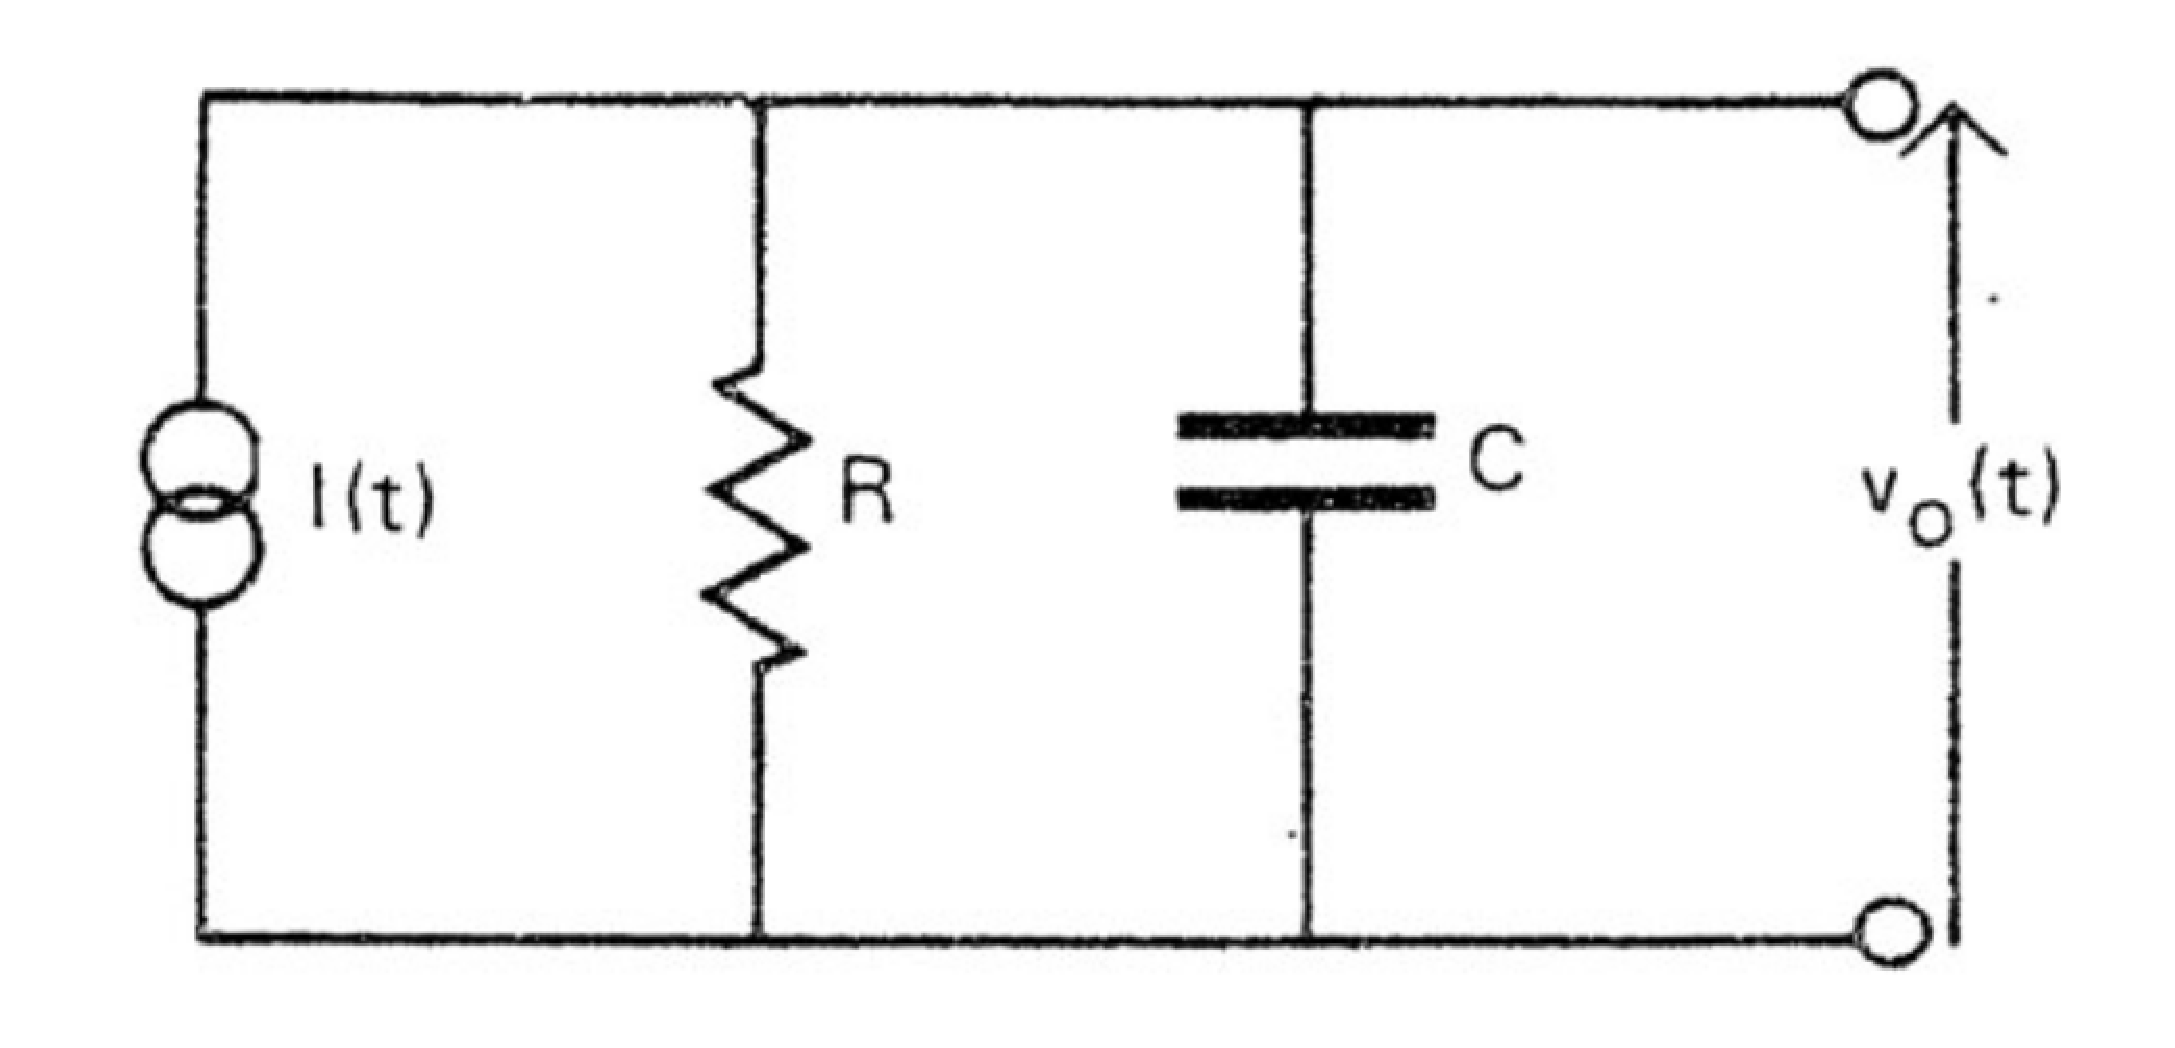
\includegraphics[width=0.6\textwidth]{d1/modelo_PMT}
\end{center}
\end{frame} 

\begin{frame}
\frametitle{Circuito equivalente y señal de salida}
\begin{itemize}
\item La mayor\'ia de las aplicaciones se pueden analizar en t\'erminos de una
combinaci\'on de R y C
\item Sin p\'erdida de generalidad, podemos tomar $R = R_0 // R_1$ y $C = C_0 + C_1$
\item Con $R_1$ y $C_1$ las resistencia y capacitancia equivalentes del circuito
de carga
\end{itemize}
\begin{center}
\includegraphics[width=0.7\textwidth]{d1/modelo2_PMT}
\end{center}
\end{frame} 

\begin{frame}
\frametitle{Circuito equivalente y señal de salida}
\begin{block}{}
Consideremos un pulso de luz de salida con decaimiento exponencial en la
intensidad (t\'ipico de un centellador, por ejemplo), con una constante
de tiempo $\tau_s$. La corriente de $pe^-$, $I(t)$, viene dada por
$$I(t) = \frac{GNq}{\tau_s}\, e^{(-t/\tau_s)} \quad \text{con}\,N = Nº\,\text{
total de}\,\, pe^- $$

Tenemos entonces una ecuaci\'on de la forma 
$$I(t) = \frac{V}{R} + C \frac{dV}{dt}$$

\end{block}
\end{frame} 

\begin{frame}
\frametitle{Circuito equivalente y señal de salida}
\begin{block}{}
Las posibles soluciones ($\tau = RC$)
$$V(t) = - \frac{GNqR}{\tau - \tau_s}\left[e^{(-t/\tau_s)} -
e^{-t/\tau}\right]\qquad \tau \neq \tau_s$$
$$V(t) = - \frac{GNqRt}{\tau_s^2}\,e^{(-t/\tau_s)} \qquad \tau = \tau_s$$
o en funci\'on de $C$
$$V(t) = - \frac{GNqt}{(C \tau_s)}\, e^{(-t/\tau_s)} \qquad \tau = \tau_s$$
\end{block}
\end{frame} 

\begin{frame}
\frametitle{Circuito equivalente y señal de salida}
\begin{columns}
\begin{column}{0.5\textwidth}
\begin{center}
\footnotesize{{\color{blue}$R = 50\,\Omega$ y $C$ variable ($\tau_s = 5\,ns$)}}
\includegraphics[width=1.1\textwidth]{d1/ec3_informe}
\end{center}
\end{column}
\begin{column}{0.5\textwidth}
\begin{center}
\footnotesize{{\color{blue}$C = 10\,pF$ y $R$ variable ($\tau_s = 5\,ns$)}}
\includegraphics[width=1.1\textwidth]{d1/ec3R_informe}
\end{center}
\end{column}
\end{columns}
\end{frame}

\begin{frame}
\frametitle{Circuito equivalente y señal de salida}
Podemos sacar algunas conclusiones:
\begin{itemize}
\item La m\'axima amplitud de se\~nal se obtiene para $R \to \infty$. En este
        caso la corriente $I(t)$ simplemente estar\'a cargando el capacitor $C$ y
        la tensi\'on de salida ser\'a

      $$V_o(t) = - \frac{GNq}{C}\, [e^{(-t/\tau_s)} - 1]$$ 

\item Solamente cuando $\tau << \tau_s$ el voltaje de salida ser\'a una 
        reproducci\'on de la corriente $I(t)$ de entrada.
\item El \'area bajo los pulsos es la misma y proporcional a $GNq$.
\item Al considerar el caso $\tau = \tau_s$; cuando $I(t)$ ha deca\'ido dentro
del 1\% de su
      valor inicial, $V(t)$ es todav\'ia $\sim$ 10\% de $V_{max}$. En otras
palabras, el
      pulso de salida tendr\'a un decaimiento largo, que aumenta con $\tau$.
\end{itemize}
\end{frame} 

\begin{frame}
\frametitle{Circuito equivalente y señal de salida}
Podemos sacar algunas conclusiones (cont.):
\begin{itemize}
\item Cuando $R \leq 100\,\Omega$, lo que implica $\tau << \tau_s$, el pulso no
      se integra - esto se denomina {\color{blue}``funcionamiento en modo corriente''} -,
      con el tiempo de subida de los pulsos de corriente y de tensi\'on
      determinado principalmente por la mayor constante de tiempo. Con $\tau
      >> \tau_s$, el pulso de corriente se integra y esta forma de
      funcionamiento se denomina {\color{blue}``modo de tensi\'on''}. Se puede notar c\'omo
      el tiempo de subida (rise time) aumenta a medida que se alcanza el
      ``modo de tensi\'on'' y, en el caso extremo, con $\tau \to \infty$, el 
      tiempo de subida de la tensi\'on es igual al tiempo de decaimiento de la
      entrada.
\item Una constante de tiempo larga es adecuada para bajas tasas de eventos. Si
      la tasa de eventos es $\sim 1/\tau$, ocurre el fen\'omeno de
      acumulamiento (``pulse pile-up'').
\end{itemize}
\end{frame} 

\subsection{Modos de operaci\'on}

\begin{frame}
\frametitle{Modos de operaci\'on}
\begin{columns}
\begin{column}{0.60\textwidth}
\begin{block}{}
\begin{itemize}
\item Pulsada o digital
\begin{itemize}
\item Photon counting
\item Es la m\'as demandante
\item No funciona bien cuando la intensidad de los fotones incidentes es muy alta y la
electr\'onica asociada no es lo suficientemente r\'apida
\item Funciona mejor cuando los fotones incidentes est\'an bien separados temporalmente
\item El n\'umero de pulsos es proporcional a la intensidad de la luz incidente  
\item {\color{blue}La altura de los pulsos no es la misma $\rightarrow$ responde al hecho de
que el proceso de multiplicaci\'on de $e^-$ es un fen\'omeno estoc\'astico}
\end{itemize}

%\item Cont\'inua o anal\'ogica 
%\begin{itemize}
%\item 
%\end{itemize}
\end{itemize}
\end{block}
\end{column} 
\begin{column}{0.40\textwidth}
\begin{center}
\fbox{\includegraphics[width=0.9\textwidth]{d1/photon_counting_mode}}
\end{center}
\end{column}
\end{columns}
\end{frame} 

\begin{frame}
\frametitle{Modos de operaci\'on}
\begin{columns}
\begin{column}{0.60\textwidth}
\begin{block}{}
\begin{itemize}
%\item Pulsada o digital
%\begin{itemize}
%\item Photon counting
%\item Es la m\'as demandante
%\item Requiere electr\'onica r\'apida
%\item Funciona mejor cuando los fotones incidentes est\'an bien separados temporalmente
%\end{itemize}

\item Cont\'inua o anal\'ogica 
\begin{itemize}
\item Se da cuando la frecuencia de arribo de los pulsos es grande y la
electr\'onica no puede diferenciar entre pulsos sucesivos 
\item Es una consecuencia del pulse pile-up (acumulamiento)
\item En este modo aparece una corriente media que tiene caracter\'isticas
t\'ipicas de ruido shot
\end{itemize}
\end{itemize}
\end{block}
\end{column} 
\begin{column}{0.40\textwidth}
\begin{center}
\fbox{\includegraphics[width=0.9\textwidth]{d1/analog_mode}}
\end{center}
\end{column}
\end{columns}
\end{frame} 

\subsection{Redes de polarizaci\'on}

\begin{frame}
\frametitle{Red de polarizaci\'on}
\begin{itemize}
\item Requerido para acelerar y enfocar correctamente los electrones
\item Establece los gradientes de potencial requeridos entre etapas (d\'inodos) 
\item {\color{blue}Mayor potencial en el \'anodo}
\item Compuesto por una cadena de $R$ (tambi\'en puede haber $C$ y transistores)
\item {\color{blue}Su configuraci\'on determina el rango din\'amico, la linealidad y la ganancia
que tendr\'a nuestro detector}
\item La fuente de alimentaci\'on debe ser estable
\end{itemize}
\begin{center}
\fbox{\includegraphics[width=0.4\textwidth]{d1/tapered_menor_v_last_dyn}}
\end{center}
\end{frame}

\begin{frame}
\frametitle{Red de polarizaci\'on}
\framesubtitle{Red pasiva}
\only<1>{\begin{center}
\fbox{\includegraphics[width=0.9\textwidth]{d1/tapered_bleeder_circuit}}
\end{center}}
\only<2>{\begin{block}{}
La corriente de la red (\alert{bleeder current}) debe ser mucho mayor que la
corriente del tubo

La variaci\'on de ganancia viene dada por 

$$\frac{\Delta G}{G} = \frac{I_{an}}{I_{bl}}\frac{n(1-\delta) +
1}{(1+n)(1-\delta)}$$

$I_{an} \rightarrow$ corriente media de \'anodo 

$I_{bl} \rightarrow$ corriente de purga (bleeder) 

$n \rightarrow$ n\'umero de etapas

$\delta \rightarrow$ factor de emisi\'on secundario
\end{block}}
\end{frame}

\begin{frame}
\frametitle{Red de polarizaci\'on}
\framesubtitle{Red activa}
\begin{center}
\fbox{\includegraphics[width=0.9\textwidth]{d1/red_divisora_activa}}
\end{center}
\end{frame}

%\begin{frame}
%\frametitle{La influencia de los capacitores de acople}
%\begin{columns}
%\begin{column}{0.50\textwidth}
%\begin{block}{Electr\'onica dedicada para Auger}
%\begin{itemize}
%\item Poco flexible 
%\item Informaci\'on limitada
%\item N\'umero limitado de UBs (\alert{Unified Boards})
%\item Comunicaci\'on de datos por puerto serie
%\item	Tiempos de adquisici\'on largos
%\item	Poco volumen de almacenamiento
%\item Sin control l\'inea de base	
%\end{itemize}
%\end{block}
%\end{column} 
%\begin{column}{0.50\textwidth}
%\fbox{\includegraphics[width=\textwidth]{d1/pmt_esquema}}
%\end{column}
%\end{columns}
%\end{frame} 

\subsection{C\'alculo de la corriente media de \'anodo}

\begin{frame}
\frametitle{C\'alculo de la corriente media de \'anodo}
\framesubtitle{La corriente de \'anodo}
\begin{block}{}
\begin{itemize}
\item $\bar{I}_a$ importa en el diseño de la red de polarizaci\'on
\item Determina el rango de trabajo donde se asegura cierto grado de
linealidad del circuito
\item Corresponde al producto de la carga por pulso, $Q$, y la
frecuencia de pulsos (que es la misma que la tasa de conteo), $f_p$
$$\bar{I}_a = Q f_p$$
\item Para asegurar variaciones de tensi\'on m\'inimas, $I_{bl}$ debe ser:
$$I_{bl}/\bar{I}_a \geq 100$$ 
\end{itemize}
\end{block}
\end{frame} 

\begin{frame}
\frametitle{C\'alculo de la corriente media de \'anodo}
\framesubtitle{Teor\'ia de diseño}
\begin{columns}
\begin{column}{0.5\textwidth}
\begin{itemize}
\item N electrones por segundo generan una $I_k$ 
\item $I_k$ aparece como una corriente de salida, luego de ser amplificada por 3
etapas con ganancia $\delta$ cada una
\end{itemize}
\end{column}
\begin{column}{0.5\textwidth}
\begin{center}
\includegraphics[width=\textwidth]{d1/voltage_div_3_dyn}
\end{center}
\end{column}
\end{columns}
\begin{itemize}
\item Un incremento en $I_k$ causa una ca\'ida $\Delta V$ entre $d_3$ y el \'anodo
\item Debido a que la $V_{total}$ es constante, $\Delta V$ aparece como un
incremento positivo en las etapas iniciales $d_1$ y $d_2$
\item El efecto se traduce como una variaci\'on en la $G_{total}$ del dispositivo
\item \alert{La clave en el diseño del divisor radica en minimizar ese efecto de
realimentaci\'on}
\end{itemize}
\end{frame} 

\begin{frame}
\frametitle{C\'alculo de la corriente media de \'anodo}
\framesubtitle{Teor\'ia de diseño}
Hay dos casos:
\begin{enumerate}
\item Aplicaciones con corriente directa (modo corriente)
\item Aplicaciones pulsadas
\end{enumerate}
\only<1>{\begin{center}
\includegraphics[width=0.5\textwidth]{d1/currents_in_pmt_blanco}
\end{center}}

\only<2>{{\color{blue}Caso 1:}
\begin{itemize}
\item Si $I_k$ es cont\'inua o de variaci\'on lenta, entonces, para un tubo de $n$
etapas: $$I_{bl} - I_k \delta^n = I_{bl} - I_a \approx I_{bl}$$
\item Satisfacer la ec. anterior asegura que las tensiones inter-d\'inodo y por lo
tanto la ganancia permanecer\'an constantes para $I_a \leq I_{a\, max}$
\end{itemize}}
\only<3>{{\color{blue}Caso 2:}
\begin{itemize}
\item Si $\hat{i}_a$ es una corriente transitoria, resulta necesario mantener
constantes las tensiones inter-d\'inodo por un tiempo igua a la duraci\'on de
$\hat{i}_a$ 
\item Esto puede hacerse colocando $C$ de desacople para entregar la $Q$
requerida por lo pulsos
\item Entonces 
 $$I_{bl} \ll \hat{i}_a \text{, siempre que}\,\, I_{bl} \gg \bar{I}_a$$
\item Donde $\bar{I}_a$ es la corriente media derivada de $\hat{i}_a$ integrada
en un determinado per\'iodo de tiempo 
\end{itemize}}
\end{frame} 

\subsection{Consideraciones generales}

\begin{frame}
\frametitle{Consideraciones generales}
\framesubtitle{Estabilidad en la ganancia, cambio en la tasa de conteo}
\begin{columns}
\begin{column}{0.60\textwidth}
%\begin{block}{Cambios en la ganancia}
\alert{Cambios en la ganancia}
\begin{itemize}
\item Se puede producir por efecto \alert{fatiga} $\rightarrow$ debido
principalmente a cambios en la cadena de amplificaci\'on
\item Se pueden distinguir dos tipos de cambios:
\begin{itemize}
\item \textbf{drift} $\rightarrow$ cambio en el tiempo bajo un nivel constante
de iluminaci\'on  
\item \textbf{shift} $\rightarrow$ cambio repentino en la ganancia luego de un
cambio en la corriente (ejemplo: cambio en la ganancia debido a un cambio en la
tasa de conteo)
\end{itemize}
\end{itemize}
%\end{block}
\end{column} 
\begin{column}{0.40\textwidth}
\begin{center}
\includegraphics[width=\textwidth]{d1/shift_and_drift_pmt}
\end{center}
\end{column}
\end{columns}
\end{frame} 

\begin{frame}
\frametitle{Consideraciones generales}
\framesubtitle{Estabilidad en la ganancia, cambio en la tasa de conteo}
\only<1>{Para probar la estabilidad de un PMT se puede usar el siguiente m\'etodo:

Montar el PMT con un sistema de centelleo y un analizador multicanal. Observar
la distribuci\'on de amplitudes de una fuente de $^{137}{Cs}$. En particular notar
la posici\'on del pico de $662\,keV$}

\only<2>{\textbf{Para medir drift} 
\small{\begin{enumerate}
\item Ajustar la distancia de la fuente tal que la tasa de conteo sea $\approx
1000\,s^{-1}$
\item Dejar que el PMT opere con esa tasa por 3 horas
\item Luego una vez cada hora por unas 20 horas, determinar la posici\'on del pico
\end{enumerate}
El drift viene dado por: $$\text{DRIFT} = \frac{\sum_i |\overline{P} -
P_i|}{n\overline{P}}$$

$P_i \rightarrow$ i-\'esima medici\'on del pico

$n \rightarrow$ n\'umero de mediciones

$\overline{P} \rightarrow$ promedio de $P_i$ sobre todas las $n$ mediciones

\alert{Para un PMT aceptable, el drift no debe superar el 1\%}}}

\only<3>{\textbf{Para medir shift} 
\small{\begin{enumerate}
\item Inmediatamente despu\'es de medir el drift, reducir la distancia de la
fuente tal que la tasa de conteo sea $\approx 10000\,s^{-1}$
\item Anotar la medici\'on del pico cada 10 min. para 4 o 5 mediciones
\end{enumerate}
El shift viene dado por: $$\text{SHIFT} = \sum_i \frac{|P_i - P_n|}{mP_n}$$

$P_n \rightarrow$ la \'ultima medici\'on hecha para el drift a 1000 cuentas/s

$P_i \rightarrow$ i-\'esima medici\'on hecha para shift

$m \rightarrow$ n\'umero de mediciones

\alert{Para un PMT aceptable, el shift no debe superar el 1\%}}}
\end{frame}

\begin{frame}
\frametitle{Consideraciones generales}
\framesubtitle{Distribuci\'on de amplitudes}
\begin{center}
\fbox{\includegraphics[width=0.5\textwidth]{d1/pulse_height_distribution_pmt}}
\end{center}
Distribuci\'on de altura de pulsos de \'anodo observados. En un experimento de
conteo de fotones (photon counting) la mejor SNR se obtiene colectando
\'unicamente los pulsos cuyas amplitudes se encuentran entre la regi\'on sombreada
AB.  
\end{frame}

\begin{frame}
\frametitle{Consideraciones generales}
\framesubtitle{Ruido en los PMTs}
\begin{block}{Variadas fuentes}
\begin{itemize}
\item Emisi\'on termoi\'onica del fotoc\'atodo
\item Emisi\'on termoi\'onica de los d\'inodos
\item Emisi\'on por campos altos inter-d\'inodos
\item Materiales radiactivos en la envoltura del PMT (p. ej. $^{40}K$ en el
vidrio) 
\item $e^-$ golpeando la envoltura del tubo y causando fluorescencia 
\item $e^-$ golpeando los d\'inodos y causando fluorescencia 
\item Rayos c\'osmicos
\end{itemize}
\end{block}
\end{frame}

\begin{frame}
\frametitle{Consideraciones generales}
\framesubtitle{Ajuste del voltaje del PMT: Plateau}
\begin{columns}
\begin{column}{0.5\textwidth}
\begin{itemize}
\item El voltaje aplicado al PMT determina su ganancia y entonces la altura de
los pulsos de salida
\item A veces es necesario ajustar la tensi\'on aplicada teniendo en cuenta
efectos de saturaci\'on o de corrientes excesivas
\end{itemize}
\end{column}
\begin{column}{0.5\textwidth}
\begin{center}
\includegraphics[width=0.5\textwidth]{d1/plateau}
\end{center}
\end{column}
\end{columns}
\end{frame}

\begin{frame}
\frametitle{Consideraciones generales}
\framesubtitle{Ajuste del voltaje del PMT: Plateau}
\begin{columns}
\begin{column}{0.5\textwidth}
\begin{itemize}
\item Es un procedimiento usado para encontrar el voltaje de trabajo adecuado en
photon counting 
\item Representa la zona en la que el conteo es menos sensible a cambios de
voltaje 
\item La segunda ``subida'' marca el efecto de regeneraci\'on (afterpulsos,
descargas, etc)
\end{itemize}
\end{column}
\begin{column}{0.5\textwidth}
\begin{center}
\includegraphics[width=0.9\textwidth]{d1/plateau2}
\end{center}
\end{column}
\end{columns}
\end{frame}

\begin{frame}
\frametitle{Consideraciones generales}
\framesubtitle{Señal del \'ultimo d\'inodo}
\begin{block}{Se elige la señal del \'ultimo d\'inodo debido a que:}
\begin{itemize}
\item La señal del d\'inodo se produce simult\'aneamente con la
salida del \'anodo, de modo que se puede utilizar como
señal de temporizaci\'on de eventos.
\item Puede utilizarse en conjunto con la señal del \'anodo para
extender el rango din\'amico de la medici\'on.
\item La señal tomada del \'ultimo d\'inodo tiene una amplitud
comparable con la del \'anodo y tiene una mayor relaci\'on
señal/ruido que los otros d\'inodos.
\item La señal del \'ultimo d\'inodo tiene polaridad opuesta a la
del \'anodo.
\end{itemize}
\end{block}
\end{frame}

%------------------------------------------------------------------------------
\section{Los fotomultiplicadores de silicio (SiPM)}
%------------------------------------------------------------------------------

\begin{frame}
\begin{center}
\Huge{\color{blue}{Los SiPM (o MPPC)}} \\
\begin{center}
\fbox{\includegraphics[width=0.8\textwidth]{d1/sipm_portada}}
\end{center}
\end{center}
\end{frame}

\begin{frame}
\frametitle{Introducci\'on}
\begin{block}{}
\begin{itemize}
\item Los MPPC son un nuevo tipo de dispositivos para el conteo de fotones
compuestos por m\'ultiples p\'ixels de APD (avalanche
photodiode) funcionando en modo Geiger
\item Son esencialmente dispositivos opto-semiconductores con excelentes
capacidades de conteo de fotones
\item Tienen ventajas respecto a otros dispositivos, tal como el bajo voltaje de
operaci\'on y la insensibilidad a los campos magn\'eticos 
\end{itemize}
\end{block}
\begin{center}
\includegraphics[width=0.4\textwidth]{d1/sipm_varios}
\end{center}
\end{frame}

\begin{frame}
\frametitle{Introduction}
\begin{block}{Outstanding features}
\begin{itemize}
\item Excellent photon counting capacity (excellent eficiency of detection vs.
number of incident photons)
\item Size
\item Operation at laboratory temperatures
\item Low working voltages (below 80 V)
\item High gain: $10^5$ a $10^6$
\item Excellent temporal resolution
\item Insensitive to magnetic fields
\item Simple electronic readout
\end{itemize}
\end{block}
\end{frame}

\begin{frame}
\frametitle{Operating principle}
\framesubtitle{Geiger mode}
\begin{center}
\includegraphics[width=0.8\textwidth]{d1/curva_sipm}
\end{center}
\end{frame}

\begin{frame}
\frametitle{Operating principle}
\framesubtitle{Structure}
\begin{center}
\fbox{\includegraphics[width=0.9\textwidth]{d1/sipm_operation}}
\end{center}
\end{frame}

\begin{frame}
\frametitle{Structure}
\framesubtitle{Photon counting}
\begin{center}
\fbox{\includegraphics[width=0.5\textwidth]{sipm_con_pulsos}}
\end{center}
\end{frame}

\subsection{The equivalent circuit of the MPPC}

\begin{frame}
\frametitle{Operating principle}
\framesubtitle{Equivalent circuit}
\begin{center}
\includegraphics[width=0.5\textwidth]{d1/sipm_equiv_circ}
\end{center}

$R_q \rightarrow$ R de enfriamiento (quenching)

$C_q \rightarrow$ C par\'asita

$C_d\,\,\text{y}\,\,C_g \rightarrow$ C asociadas a la microcelda y a las
conexiones ($30-50\,\text{fF}$)
\end{frame}

\begin{frame}
\frametitle{Principio de operaci\'on}
\framesubtitle{Lectura de la señal de salida}
\includegraphics[width=0.8\textwidth]{d1/readout_sipm}
\end{frame}

\begin{frame}
\frametitle{Operating principle}
\framesubtitle{Reading the output signal}
It can be used two methods to estimate the number of photons detected by the
MPPC

\only<2>{
\alert{Observing the output pulses (amplitude)}
\begin{center}
\includegraphics[width=0.6\textwidth]{d1/pulso_sipm}
\end{center}}

\only<3>{
\alert{Measuring the output charge}
\begin{center}
\includegraphics[width=0.4\textwidth]{d1/sipm_spectrum}
\end{center}}
\end{frame}

\begin{frame}
\begin{block}{Introducci\'on (cont.)}
ATP es la molécula de energía universal que se encuentra en todo el material
orgánico. Esto incluye organismos, fluidos corporales y
residuos de alimentos. La combinación de ATP con la enzima luciferasa produce
luz que puede medirse en un luminómetro. La
cantidad de luz es proporcional a la cantidad de ATP y se expresa en Unidades
Relativas de Luz (URL). Cuanto mayor es el nivel de
ATP, mayor será el valor de las URL y más sucia la mano.

\end{block}
\end{frame} 

\begin{frame}
\frametitle{Working cycle}
%\framesubtitle{Fluorescence measurement}
\begin{center}
\fbox{\includegraphics[width=0.5\textwidth]{ciclo_de_trabajo_sipm}}
\end{center}
\end{frame}

\begin{frame}
\frametitle{Comparison with Other Detector Technologies}
%\framesubtitle{Fluorescence measurement}
\begin{center}
\fbox{\includegraphics[width=0.5\textwidth]{comparacion_otros_det}}
\end{center}
\end{frame}

\begin{frame}
\frametitle{Application examples}
\framesubtitle{Fluorescence measurement}
\begin{center}
\fbox{\includegraphics[width=0.5\textwidth]{mppc_exam1}}
\end{center}
\end{frame}

\begin{frame}
\frametitle{Application examples}
\framesubtitle{Scintillation measurement}
\begin{center}
\fbox{\includegraphics[width=0.5\textwidth]{mppc_exam2}}
\end{center}
\end{frame}

\begin{frame}
\frametitle{Application examples}
\framesubtitle{Particle measurement}
\begin{center}
\fbox{\includegraphics[width=0.5\textwidth]{mppc_exam3}}
\end{center}
\end{frame}

\begin{frame}
\frametitle{Application examples}
\framesubtitle{Flow cytometry}
\begin{block}{Wikipedia}
{\scriptsize In biotechnology, flow cytometry is a laser- or impedance-based, biophysical
technology employed in cell counting, cell sorting, biomarker detection and
protein engineering, by suspending cells in a stream of fluid and passing them
through an electronic detection apparatus.} 
%A flow cytometer allows simultaneous
%multiparametric analysis of the physical and chemical characteristics of up to
%thousands of particles per second.
\end{block}
\begin{center}
\fbox{\includegraphics[width=0.4\textwidth]{mppc_exam4}}
\end{center}
\end{frame}

\begin{frame}
\begin{block}{Introducci\'on (cont.)}
Se utiliza la medición de ATP:
\begin{enumerate}
\item Como una herramienta de formación para demostrar la eficacia de una buena
técnica de lavado de manos.
\item Como una herramienta de monitoreo para medir la eficacia del lavado de manos
al hisopar las manos
limpias inmediatamente después del lavado (antes que las manos entren en
contacto con cualquier cosa).
\end{enumerate}
\end{block}
\end{frame} 

%%------------------------------------------------------------------------------
%\section{Señales pulsadas en electr\'onica nuclear}
%%------------------------------------------------------------------------------
%
%\subsection{Terminolog\'ia}
%\subsection{Señales anal\'ogicas y digitales}
%\subsection{Señales r\'apidas y señales lentas}
%\subsection{El dominio de la frecuencia. Ancho de banda}
%
%%------------------------------------------------------------------------------
%\section{Transmisi\'on de señales}
%%------------------------------------------------------------------------------
%
%\subsection{Cables coaxiales}
%\subsubsection{Impedancia caracter\'istica}
%\subsubsection{Reflexiones}
%\subsubsection{Terminaci\'on de cables: adaptaci\'on de impedancias}
%\subsubsection{P\'erdidas en cables coaxiales. Distorsi\'on de pulsos}
%\subsubsection{Respuesta del cable. Distorsi\'on de pulsos}

\begin{frame}
\begin{center}
%\huge{¡Muchas Gracias!}
\includegraphics[height=0.6\textheight,width=0.65\textwidth]{logos/gracias}
\end{center}
\end{frame}

\begin{frame}
\begin{center}
\huge{¿Preguntas?}\\
\vspace{5mm}
\includegraphics[height=0.4\textheight,width=0.4\textwidth]{logos/preguntas}
\end{center}
\end{frame}


\end{document}
